\documentclass{article}
%\documentclass[a4paper,12pt]{article}
\newtheorem{thm}{Theorem}
\setlength{\oddsidemargin}{0.25in}
\setlength{\textwidth}{6in}
\setlength{\topmargin}{-0.25in}
\setlength{\headheight}{0.3in}
\setlength{\headsep}{0.2in}
\setlength{\textheight}{9in}
%\setlength{\footskip}{0.1in}
\usepackage{multirow}
\usepackage{fullpage}
\usepackage{graphicx}
\usepackage{amsthm}
\usepackage{amsmath}
\usepackage{amssymb}
\usepackage{url}
\usepackage{amsfonts}
%\usepackage{algpseudocode}
\usepackage{mathtools}
\usepackage{algorithm}
\usepackage{algpseudocode}
\newcommand{\argmin}{\arg\!\min}
\newcommand{\argmax}{\arg\!\max}



\newcommand{\quotes}[1]{``#1''}


\usepackage{hyperref}
\hypersetup{
    colorlinks=true,
    linkcolor=blue,
    filecolor=magenta,      
    urlcolor=blue,
}

% ===== ===== ===== ===== ===== % 
% New commands set by Chuck Jia
% ===== ===== ===== ===== ===== % 

\newcommand{\code}[1]{\texttt{#1}}
\newcommand{\qnum}[1]{\noindent\textcolor{blue}{\textbf{(#1)}}}
\newcommand{\ds}{\displaystyle}
\newcommand{\tx}[1]{\text{#1}}
\newcommand{\ba}{\[\begin{aligned}}
\newcommand{\ea}{\end{aligned}\]}
\newcommand{\sep}{\begin{center}\textcolor{gray}{\rule{\textwidth}{0.75pt}}\end{center}}
\usepackage{minted}
\usepackage{color}
\usepackage{xcolor}
\definecolor{myorange}{RGB}{255, 165, 0}
\definecolor{mydarkgreen}{RGB}{0, 100, 0}
\definecolor{mybrickred}{RGB}{132, 31, 39}
\definecolor{myfirebrick}{RGB}{178, 34, 34}

\usepackage{booktabs}
\usepackage{array}


\begin{document}\title{Homework 4\\ Applied Machine Learning \\ Fall 2017\\ CSCI-P 556/INFO-I 526}         % Enter your title between curly braces
\author{Chuck Jia}        % Enter your name between curly braces
\date{November 28, 2017}          % Enter your date or \today between curly braces
\maketitle
\quotes{All the work herein is solely mine.}
\makeatother     % `@' is restored as a "non-letter" character
\pagestyle{plain}
\section*{Directions}
Please follow the syllabus guidelines in turning in your homework.  I am providing the \LaTeX{} of this document too. This homework is due Monday November 20, 2017 11:59p.m. \textbf{OBSERVE THE  TIME}. Absolutely
no homework will be accepted after that time. Bring a hardcopy to Tuesday’s class on the 21th.
If you do not bring a hardcopy with the statement of your own work, the homework will not be
accepted. All the work should be your own.  Within a week, AIs can contact students to examine code; students must meet within three days.  The session will last no longer than 5 minutes.  If the code does not work, the grade for the program may be reduced.  Lastly, source code cannot be
 modified post due date.
 
 
 
  
\section*{K-Fold Cross Validation for Model Selection }

{\small
\begin{center}
\begin{algorithmic}[1]\label{alg:crossValidation}
\State{\bf ALGORITHM} \texttt{k-fold cross validatiaon}
\State {\bf INPUT} \begin{itemize}
\item \textsf{training data} $\Delta = (\mathbf{x_1},y_1),\ldots,(\mathbf{x_m},y_m)$
\item  set of parameter values $\Theta$
\item  learning algorithm $\mathcal{H}$
\item  integer $k$
\end{itemize}
\State {\bf OUTPUT}\begin{itemize}
\item $\theta^* =\argmin_\theta [error(\theta)]$
\item $h_{\theta^*} = \mathcal{H}(\Delta;\theta^*)$ 
\end{itemize}
\State Randomly partition $\Delta$ into $\Delta_1,\ldots,\Delta_k$
\State  \texttt{***} $\Delta_1\cup\Delta_2\ldots \cup\Delta_k = \Delta$ and $\Delta_i \cap \Delta_j = \varnothing$ for $i \neq j \in [1,2,\ldots,k]$
\For{$\theta \in \Theta$}
\For {$i = 1\ldots k$}
\State  \texttt{***}  \textsf{Train a model for each training set}
\State $h_{i,\theta} = \mathcal{H}(\Delta \setminus \Delta_i;\theta)$
\EndFor
\State  \texttt{***}  \textsf{Use the trained models over $\Delta_i$ (test data sets) to evaluate the models for each parameter}
\State error$(\theta)= \frac{1}{k} \sum_{i=1}^{k} \mathcal{L}_{\Delta_i} (h_{i,\theta})$
\EndFor
\end{algorithmic}
\end{center}}

\pagebreak
 
\section*{K-Nearest Neighbors (KNN) Algorithm in Theory}
{\small
\begin{center}
\begin{algorithmic}[1]\label{alg:knn}
\State{\bf ALGORITHM} \texttt{K-nearest neighbors}
\State {\bf INPUT}\begin{itemize}
\item \textsf{training data} $\Delta$
\item \textsf{test data} $\Delta'$  
\item \textsf{distance metric} $d$, i.e., $d:\Delta^2\rightarrow \mathbb{R}_{\geq 0}$ 
\item \textsf{integer} $k$: \textsf{nearest neighbors number}
\end{itemize}
\State {\bf OUTPUT} 
\begin{itemize}
\item \textsf{class label of each} $z \in \Delta' $
\end{itemize}
\For {$z = (\mathbf{x}',y') \in \Delta'$}
\State  \textsf{Compute} $d(\mathbf{x},\mathbf{x}')$, \textsf{the distance between z and every example} $(\mathbf{x},y) \in \Delta$
\State  \textsf{Select} $\Delta_z \subseteq \Delta$, \textsf{the set of closest} $k$ \textsf{training examples to z}
\State \textsf{Voting:}
\begin{itemize}
\item \textsf{majority voting}:
$y' = \argmax_v  \sum_{(\mathbf{x_i},y_i)\in\Delta_z} I(v=y_i)$
\item \textsf{distance-weighted voting}: $y' = \argmax_v  \sum_{(\mathbf{x_i},y_i)\in\Delta_z} w_i \times I(v=y_i)$ \textsf{where} $ w_i = \frac{1}{d(\mathbf{x',x_i})^2}$
\end{itemize}
\EndFor
\end{algorithmic}
\end{center}}


\vspace{30pt}

\section*{Naive Bayes Classifier}
{\small
\begin{center}
\begin{algorithmic}[1]\label{alg:naiveBayes}
\State{\bf ALGORITHM} \texttt{ Training of naive bayes classifier (continuous attributes) }
\State  \texttt{***} \textsf{training set:} $\Delta$ = $ \{ (\mathbf{x_j}, y_j)\}_{j=1}^{m}$
\For {$i=1,\ldots,k$}
\State  \texttt{***}  \textsf{class-specific subsets}
\State $\Delta_i \leftarrow \{\mathbf{ x_j} | y_j =c_i, j=1,\ldots,m\}$
\State  \texttt{***}  \textsf{size of the subsets}
\State $m_i \leftarrow | \Delta_i|$
\State  \texttt{***}  \textsf{prior probability}
\State $\hat{P}(c_i) \leftarrow m_i/m$
\State  \texttt{***}  \textsf{mean}
\State  $\hat{\mu}_i \leftarrow \frac{1}{m_i} \sum_{\mathbf{x_j}\in\Delta_i} \mathbf{x_j} $
\State  \texttt{***}  \textsf{centered data}
\State $\mathcal{Z}_i \leftarrow \Delta_i -  \mathbb{I}_{m_i} \hat{\mu}_i^T $
\State  \texttt{***}  \textsf{variance}
\State  $\hat{\sigma}_i \leftarrow \frac{1}{m_i} \mathcal{Z}_i^T \mathcal{Z}_i$
\EndFor
\State \Return {$\hat{P}(c_i), \hat{\mu}_i, \hat{\sigma}_i$ for all  $i=1,\ldots k$}
\State
\State{\bf TESTING}( $\mathbf{x}$ and  $\hat{P}(c_i), \hat{\mu}_i, \hat{\sigma}_i$, for all $i \in [1,k])$:
\State $\hat{y} \leftarrow \argmax_{c_i} \{ f(\mathbf{x} | \hat{\mu}_i, \hat{\sigma}_i)\ \hat{P}(c_i) \} $
\State \Return {$\hat{y}$}
\end{algorithmic}
\end{center}}

\pagebreak
\subsection*{M-estimate of Conditional Probability}
If the class-conditional probability for one of the attributes is zero, then overall posterior probability for the class vanishes. This problem can be addressed by using the $m$-estimate approach for estimating the conditional probability:
\begin{equation*}
P(x_i | y_j) =  \frac{n_c + m \times p}{n+m}
\end{equation*}


\begin{itemize}
\item $x_i$: training example $x_i$, \textbf{$y_j$:} class $y_j$
\item $n_c: $ number of training examples from class $y_j$ that take on the value $x_i$
\item $n:$ total number of instances from class $y_j$
\item $m:$ equivalent sample size. $m$ determines the trade-off between the prior probability $p$ and the observed probability $n_c/n$
\item $p:$ user-specified parameter. $p$ can be regarded as the prior probability of observing the attribute value $x_i$ among records with class $y_j$
\end{itemize}

\vspace{75pt}
\sep 
\vspace{10pt}

In this homework, you are asked to implement $k$-nearest neighbors (KNN), naive bayes classifier and $k$-fold cross validation for model selection. You will test/compare them over Ionosphere, car evaluation and credit approval data sets. Click on the links below to obtain the data sets.

\begin{itemize}
\item \href{https://archive.ics.uci.edu/ml/datasets/ionosphere}{
Ionosphere Data Set }
\item \href{https://archive.ics.uci.edu/ml/datasets/car+evaluation}{Car Evaluation Data Set}
\item \href{https://archive.ics.uci.edu/ml/datasets/Credit+Approval}{Credit Approval Data Set }
\end{itemize}


%%%%%%%%%%%%%%%%%%%%%%%%%%%%%%%%%%%%%%%%%%%%%%%%%%%
%                        PROBLEM 1
%
%%%%%%%%%%%%%%%%%%%%%%%%%%%%%%%%%%%%%%%%%%%%%%%%%%%5

\newpage
\section*{Problem 1: $K$-Fold Cross Validation [25 points]}

Implement $k$-fold cross validation and select $k=5$ to create $5$ training and $5$ test data sets from each data set and save these $30$ files. You will use these data sets for model comparison and parameter selection.
\sep 


The \code{R} code for creating the cross validation files is in the file \code{Prob1-CreateFiles.R}.

The files generated are stored in the folder \code{/Data/KFold}.




























%%%%%%%%%%%%%%%%%%%%%%%%%%%%%%%%%%%%%%%%%%%%%%%%%%%
%                        PROBLEM 2
%
%%%%%%%%%%%%%%%%%%%%%%%%%%%%%%%%%%%%%%%%%%%%%%%%%%%5

\newpage
\section*{Problem 2: $K$-Nearest Neighbors (KNN)[55 points]} 

\textbf{2.1}  Implement KNN algorithm with two different distance functions. You can either use existing distance functions, i.e., Euclidean  or design your own.
\\
\\
\textbf{2.2}  Use the data sets obtained in problem 1 to determine the optimal $k$  over each data set for KNN algorithm. For  $5$ different $k$ values, plot the test error for each data set.  Total number of  figures $=$ 3 (data set number) $\times$ $2$ (distance function number) $=6$. Report the best $k$  and distance function for each data set. 
\\
\\
\textbf{2.3} Use the KNN package in R for validation.
\sep 

\qnum{2.1}
In the \code{R} code, we tested 7 different distance functions. They are the natural metrics induced by the $1$-norm, 2-norm, $\cdots$, 6-norm and the $\infty$-norm in the space $\mathbb{R}^n$. The $p$-norms are defined as usual:
\[
    \|(x_1,\cdots,x_n)\|_p 
    = \left(\sum_{i=1}^n|x_i|^p\right)^{1/p}, \quad 
    \text{for } 1<p<\infty
\]
\[
    \|(x_1,\cdots,x_n)\|_\infty 
    = \max_{i=1,\cdots,n}\{|x_i|\},\quad 
    \text{for } p = \infty
\]
The distance function corresponding to the $p$-norm is defined as 
\[
    \begin{aligned}
        \tx{dist}(\textbf{x}, \textbf{y})
        = \|\textbf{x} - \textbf{y}\|_p,\quad 
        \textbf{x}, \textbf{y} \in \mathbb{R}^n
    \end{aligned}
\]

Below we only give the results from using the $1$-norm and 2-norm distance functions, as the they are the 2 best performing distance functions among all the functions tested.
\bigskip

\noindent\textbf{Data Pre-processing}
\bigskip

Because of the existence of the categorical data, which are not numerical, we need to pre-process the original data set.
In data pre-processing, we also engineer the feature scales in order to yield better result.

In our implementation, for different data types, we use the following methods for pre-processing.
\begin{itemize}
    \item \textsl{Continuous data}: We keep them in continuous form, but we center all the continuous features and scale them to standard deviation 1. This applies to both \code{Ionosphere} and \code{Credit Approval Data} sets.
    
    \item \textsl{Categorical data}: We use dummy variables to transform them to numerical data.
    
    \item \textsl{Missing data}: Since the proportion of missing data is relatively small, we replace all the \code{?} with the mean or the median of the feature where the missing data point is located.
    The use of mean or median depends on the type of the feature. If the feature is continuous, we choose to use the mean for replacement. If the feature is categorical, we use the median.
\end{itemize}



\bigskip\bigskip




\qnum{2.2}
\bigskip

\noindent\textbf{Preliminary Analysis}
\bigskip

Before we plot the final results on 5 different $k$'s, we need to find the best $k$ values.
Here, we plot the average error rates from 20 different $k$'s in order to select the best five $k$ values.

In the 3 graphs below, the \textcolor{blue}{\code{blue lines}} represent errors from using the
\textcolor{blue}{\textbf{1-norm}} distance function, 
while the \textcolor{orange}{\code{orange lines}} represent errors from using the 
\textcolor{orange}{\textbf{2-norm}} distance function.
The error bars represent the standard deviation across the 5 validation sets for each $k$ value.

\begin{center}
    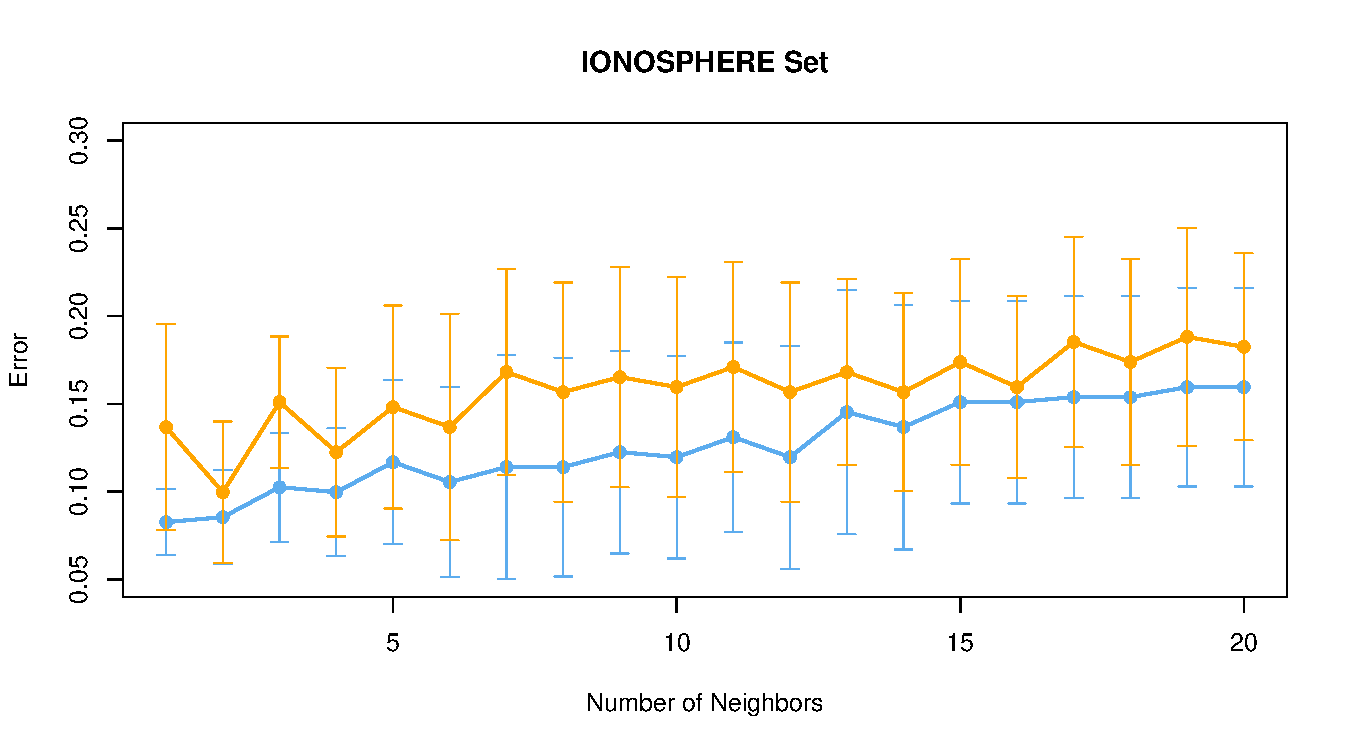
\includegraphics[width=1\linewidth]{Images/Prob2/Prob2-2-Prelim-Iono.pdf}
    \bigskip
    
    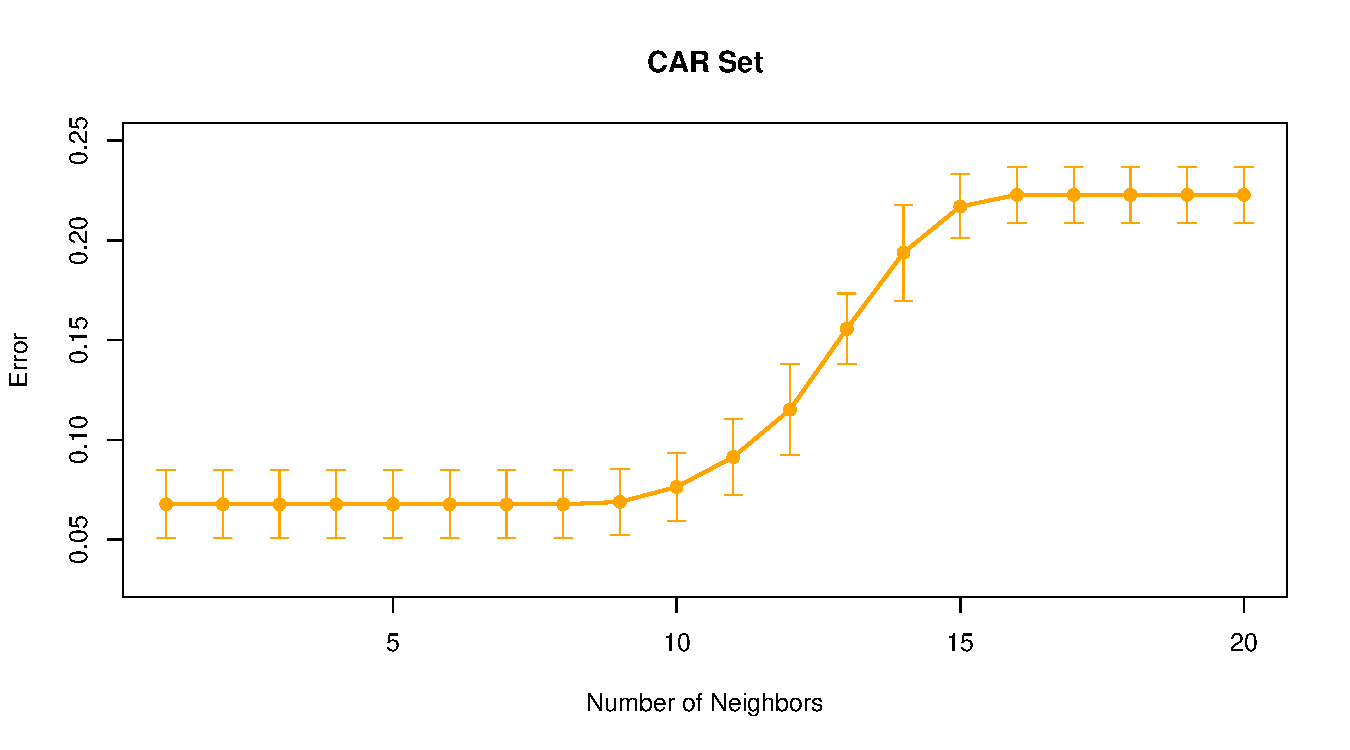
\includegraphics[width=1\linewidth]{Images/Prob2/Prob2-2-Prelim-Car.pdf}
    
    \parbox{5in}{\textit{In the car set, the results from the 2 distance functions are very similar, which results in only showing the orange line.}}\bigskip
    
    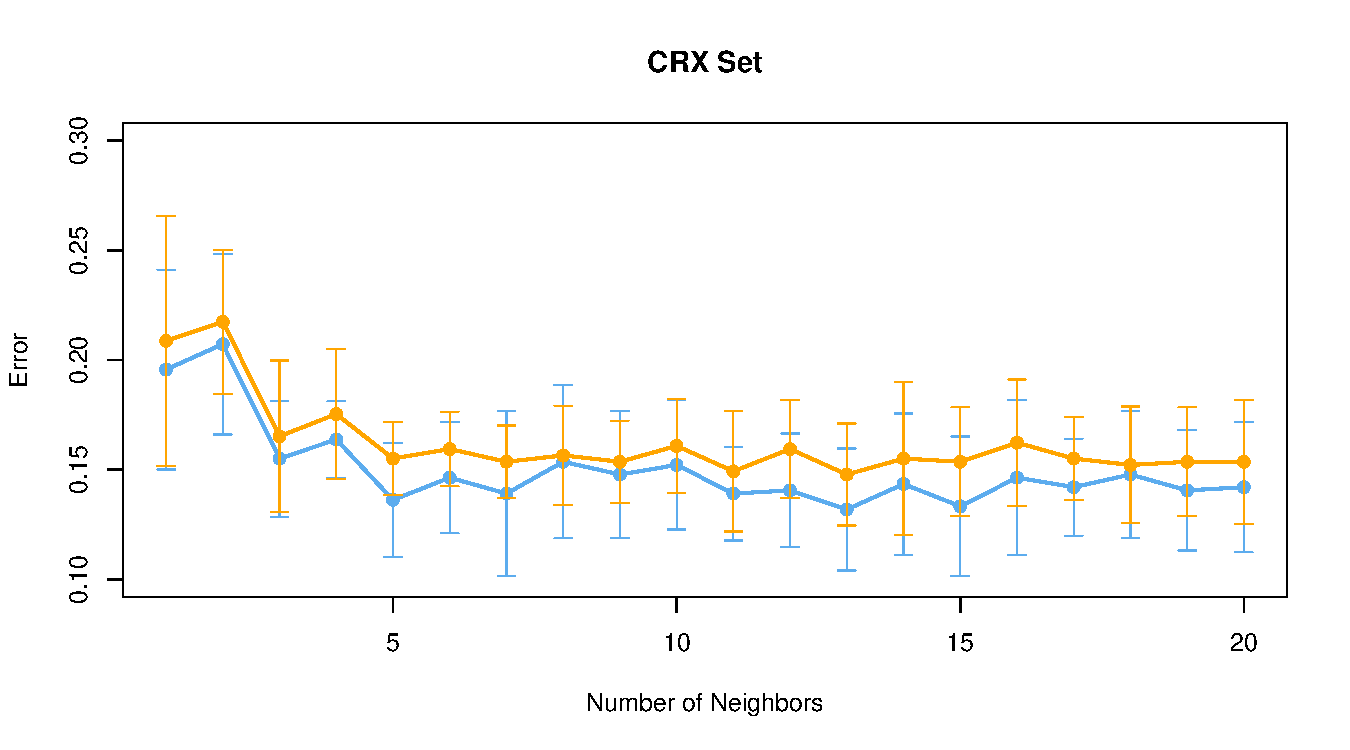
\includegraphics[width=1\linewidth]{Images/Prob2/Prob2-2-Prelim-Crx.pdf}
\end{center}
\bigskip 












\noindent\textbf{Final Results}
\bigskip

From the preliminary results above, we selected 5 best $k$ values for each data set. Now we give the error results using box plots.
\bigskip

\begin{center}
    \textcolor{mydarkgreen}{\textbf{\textsf{Ionosphere Set}}}
\end{center}


\begin{center}
    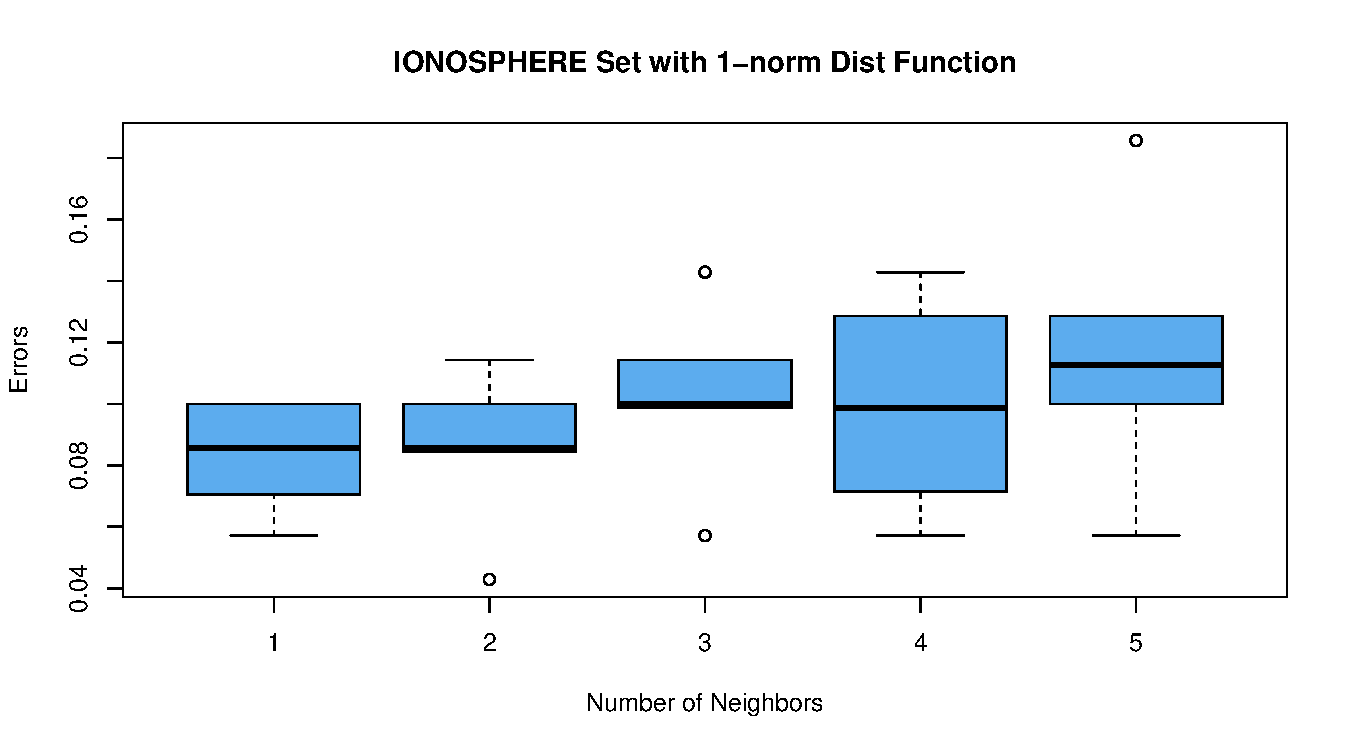
\includegraphics[width=0.9\linewidth]{Images/Prob2/Prob2-2-Iono-1norm.pdf}
    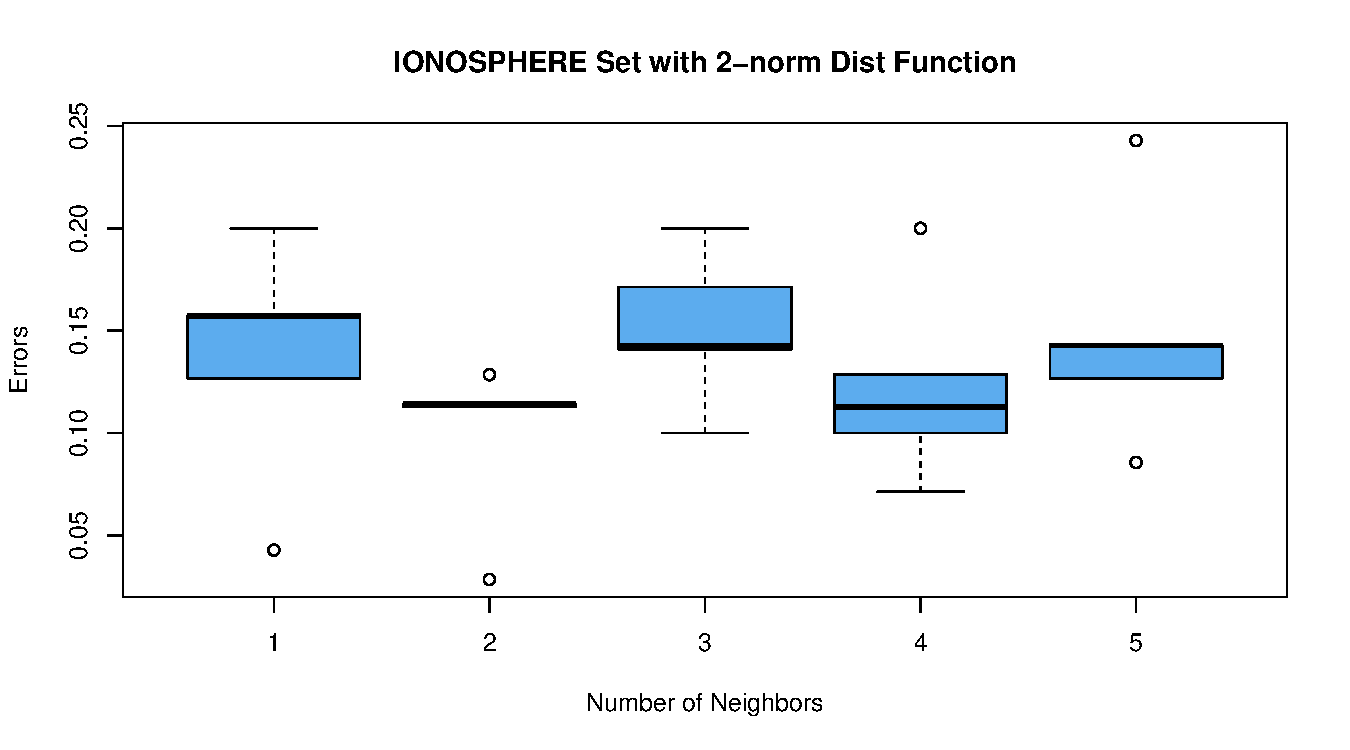
\includegraphics[width=0.9\linewidth]{Images/Prob2/Prob2-2-Iono-2norm.pdf}
\end{center}

For the Ionosphere set, the best $k$ is 1, with the 1-norm distance function. The error rate is 0.08265594.
\bigskip\bigskip

\begin{center}
    \textcolor{mydarkgreen}{\textbf{\textsf{Car Set}}}
\end{center}


\begin{center}
  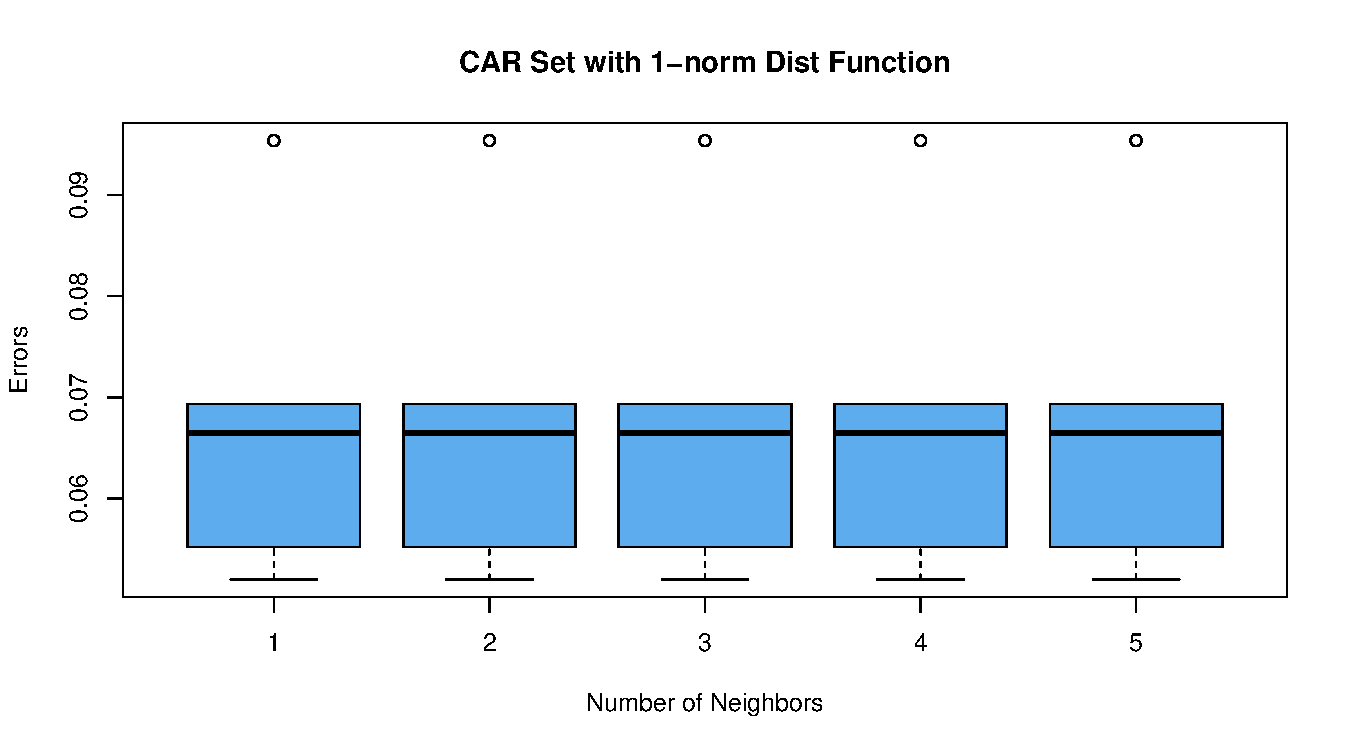
\includegraphics[width=0.9\linewidth]{Images/Prob2/Prob2-2-Car-1norm.pdf}
  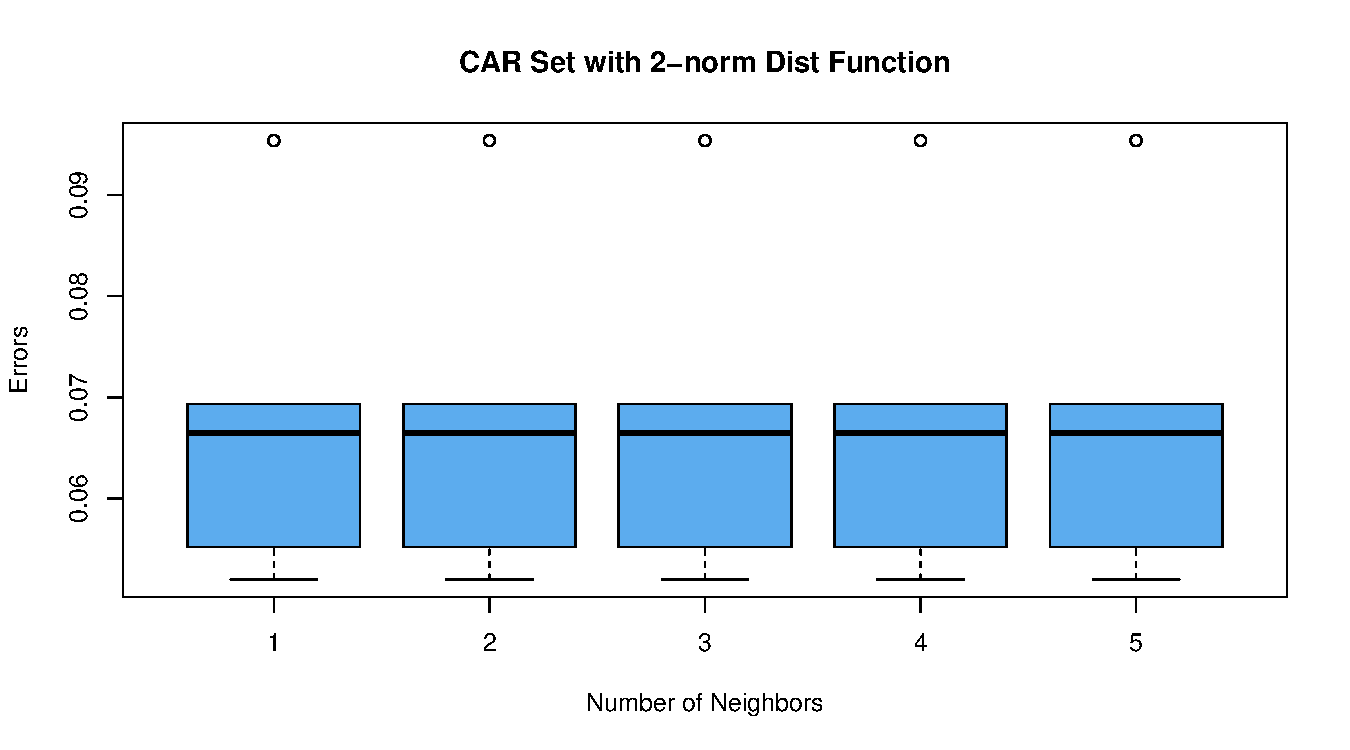
\includegraphics[width=0.9\linewidth]{Images/Prob2/Prob2-2-Car-2norm.pdf}
\end{center}

For the Car set, the best $k$ is 1, with the 1-norm distance function. The error rate is 0.06769391.

\bigskip\bigskip

\begin{center}
    \textcolor{mydarkgreen}{\textbf{\textsf{Credit Approval Data Set}}}
\end{center}

\begin{center}
  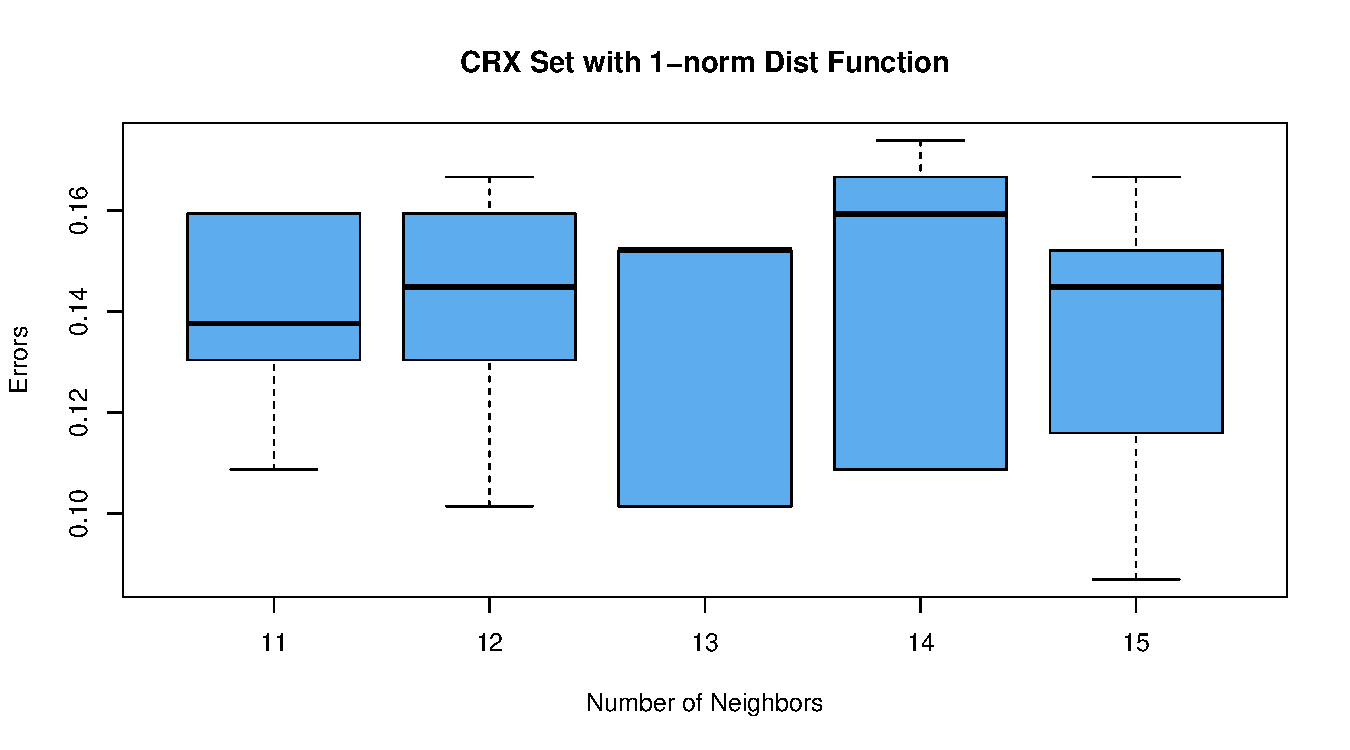
\includegraphics[width=0.9\linewidth]{Images/Prob2/Prob2-2-Crx-1norm.pdf}
  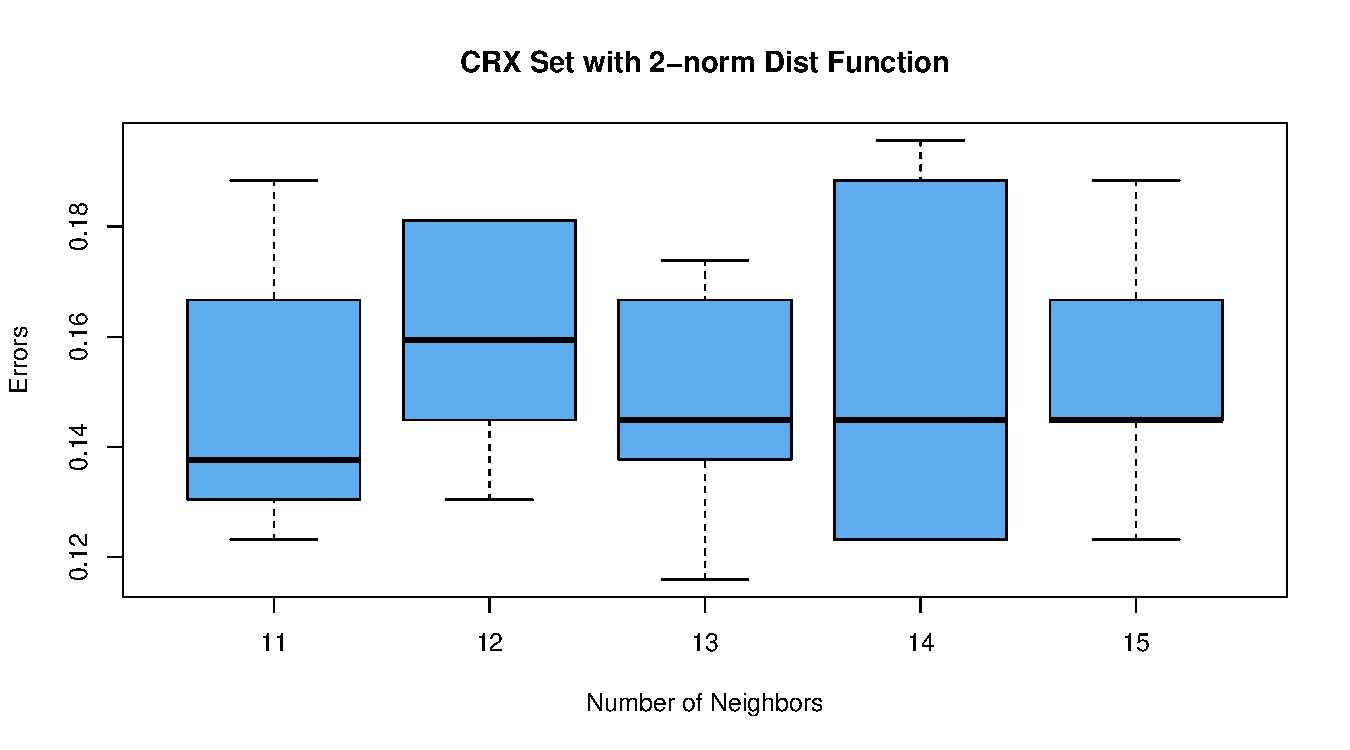
\includegraphics[width=0.9\linewidth]{Images/Prob2/Prob2-2-Crx-2norm.pdf}
\end{center}

For the Crx set, the best $k$ is 13, with the 1-norm distance function. The error rate is 0.1318841.
\bigskip \bigskip

\noindent\textbf{Summary of Results}
\bigskip

Now we summarize the best results from my implementation of KNN.

Our KNN performs best with 1-norm distance function on all of the 3 data sets. For the \code{Ionosphere} and \code{Car} sets, the best $k$ is 1, and for the \code{Credit Approval Data} set, the best $k$ is 13.
\bigskip


\begin{center}
\newcommand{\cellISize}{3cm}
\newcommand{\cellLastSize}{4.5cm}
\newcommand{\cellRowSize}{0.5cm}
\newcommand{\ci}[1]{\parbox{\cellISize}{\centering #1}}
\newcommand{\cii}[1]{& \parbox{\cellLastSize}{\centering #1}}
\newcommand{\lineend}{&\\[\cellRowSize]\hline}
\textbf{Best Average Error Rate from KNN} 
\bigskip

\begin{tabular}{m{\cellISize} | m{4.0cm} m{0cm}}
    \toprule[1.5pt]
      \centering\parbox{\cellISize}
      {\centering \textbf{Data Set}}  
      & \parbox{\cellLastSize}{\centering \textbf{Average Error Rate}} 
      &\\[0.3cm]
    \midrule[0.8pt]
    %===== ===== ===== =====%
    \ci{Ionosphere} 
    \cii{0.08265594}
    \lineend
    %===== ===== ===== =====%
    \ci{Car} 
    \cii{0.06769391}
    \lineend
    %===== ===== ===== =====%
    \ci{Credit Approval} 
    \cii{0.1318841}
    & \\[\cellRowSize]
    %===== ===== ===== =====%
    \bottomrule[1.5pt]
\end{tabular}
\end{center}
\bigskip\bigskip








\qnum{2.3}\medskip

Now we compare the results from my implementation of KNN with the results from using \code{R} built-in KNN methods for validation.

In the 3 graphs below, the \textcolor{blue}{\code{blue lines}} represent errors from using
\textcolor{blue}{\textbf{my implementation}} of KNN, 
while the \textcolor{orange}{\code{orange lines}} represent errors from using 
\textcolor{orange}{\textbf{built-in}} KNN method in R.


\begin{center}
    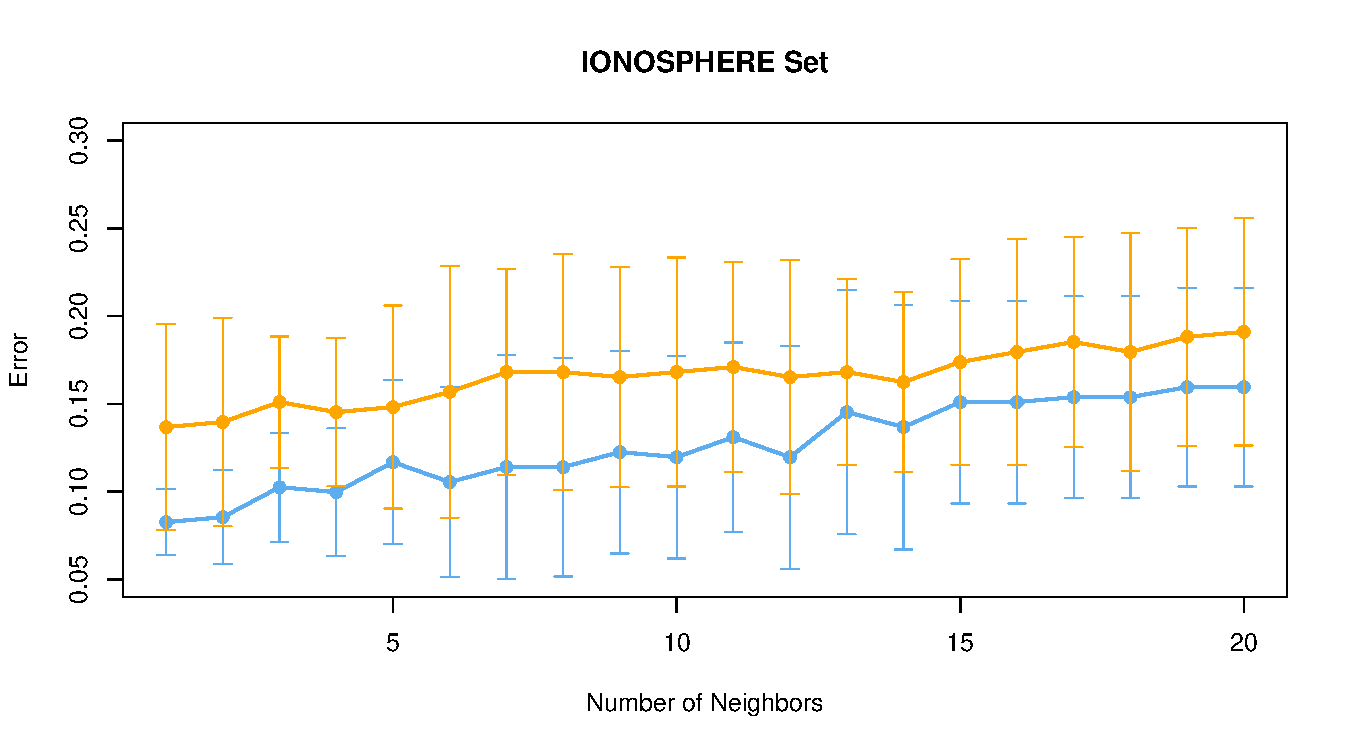
\includegraphics[width=0.9\linewidth]{Images/Prob2/Prob2-3-R_Comp-Iono.pdf}
    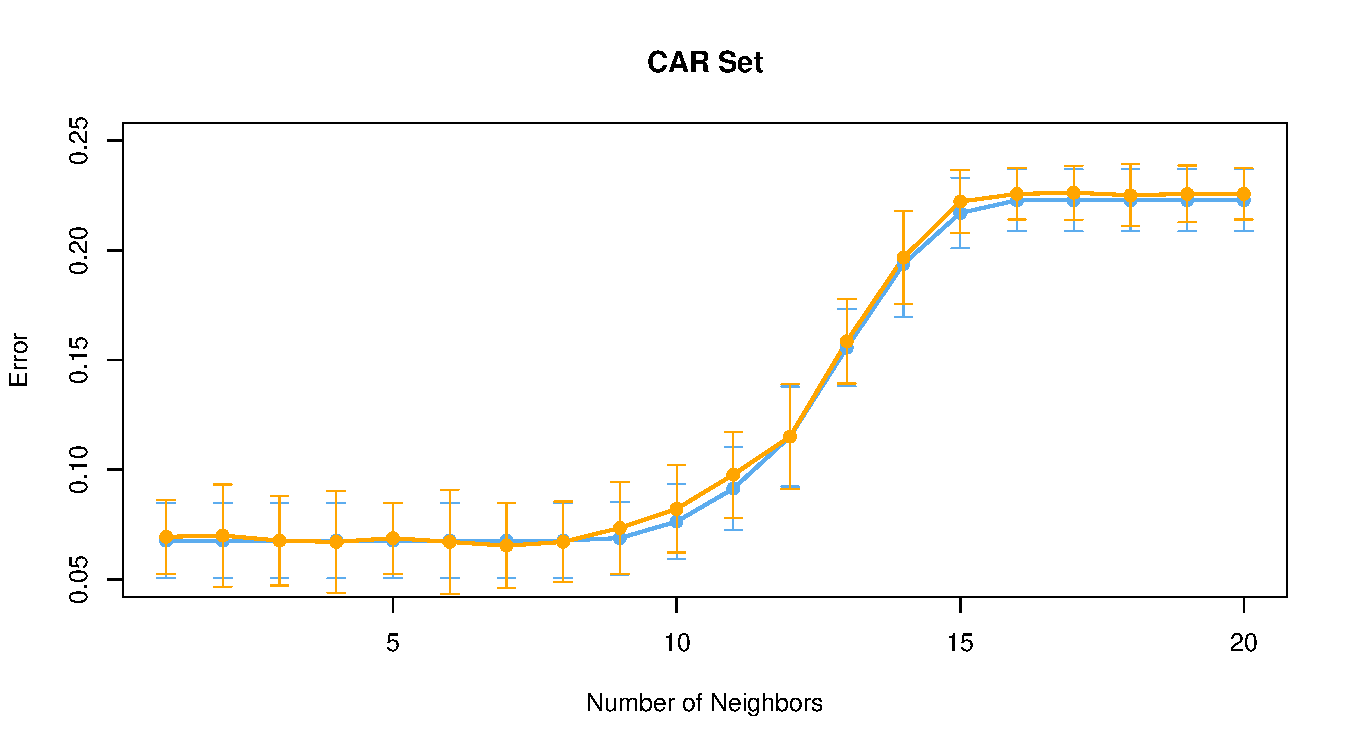
\includegraphics[width=0.9\linewidth]{Images/Prob2/Prob2-3-R_Comp-Car.pdf}
    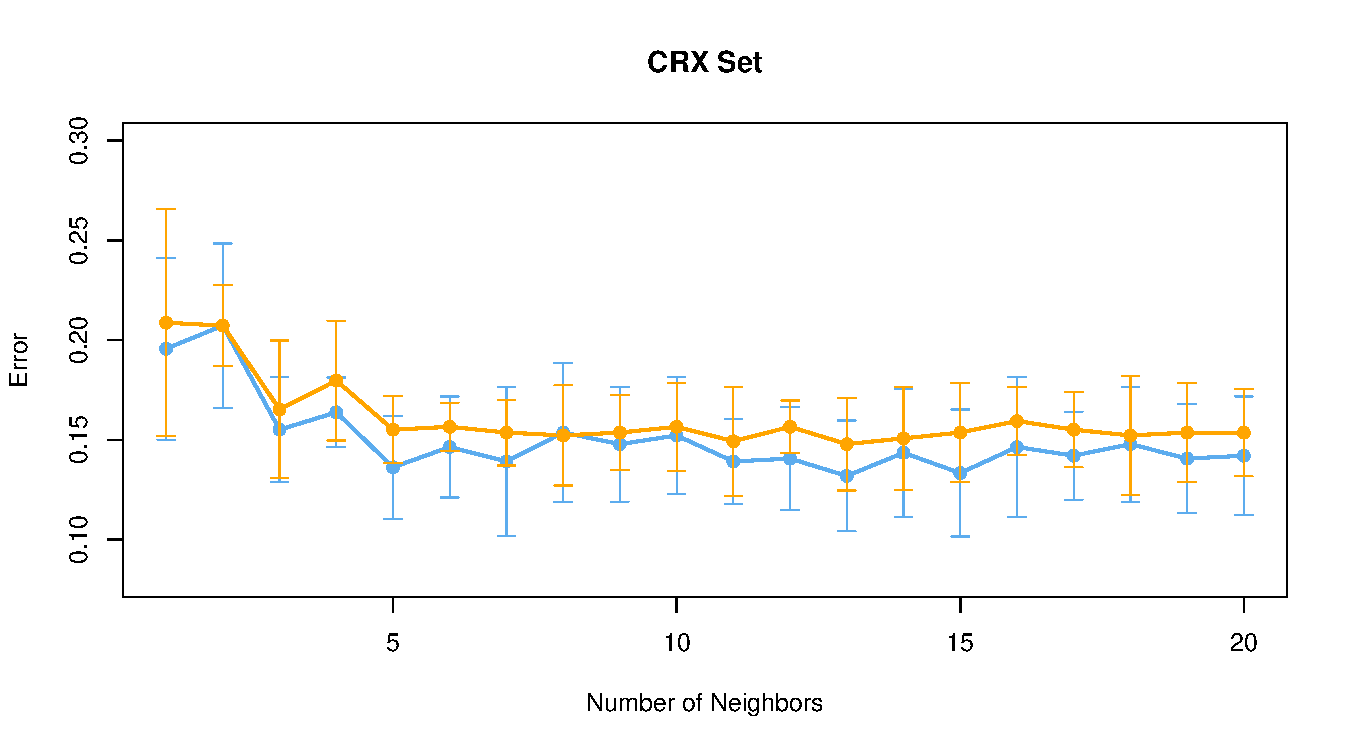
\includegraphics[width=0.9\linewidth]{Images/Prob2/Prob2-3-R_Comp-Crx.pdf}
\end{center}


As we can see, in the 2 data sets with continuous data, \code{Ionosphere} and \code{Credit Approval Data Set}, our implementation performs better than the \code{R} built-in implementation. 
The difference is in the choice of the distance function. The On these 2 data sets, the KNN method works better with the 1-norm distance function. 

In the \code{Car} data set, our implementation performs very similar with the \code{R} built-in implementation. 
This is expected, since this data set is made up of only categorical data. 
The effect of changing between 1-norm and 2-norm on discrete data is smaller than on continuous data.
The slight difference between the results from the two implementations is caused by the difference in the voting method, especially in the ways of handling ties.










































%%%%%%%%%%%%%%%%%%%%%%%%%%%%%%%%%%%%%%%%%%%%%%%%%%%
%                        PROBLEM 3
%
%%%%%%%%%%%%%%%%%%%%%%%%%%%%%%%%%%%%%%%%%%%%%%%%%%%
\newpage
\section*{Problem 3: Naive Bayes Classifier [55 points]} 
	
\textbf{3.1} Implement Naive Bayes classifier. The Pseudo-code for naive bayes algorithm is provided above. You may need to modify it for categorical variables. To handle unseen feature values, you may need to make use of $m$-estimate of conditional probability method. There are also other techniques, i.e., Laplace smoothing.
\\
\\
\textbf{3.2} Train Naive Bayes classifiers over training data sets and test each classifier against corresponding test data. Make a plot that shows the error over each test data. Report the average error rate for $5$-fold cross validation for each data sets.
\\
\\
\textbf{3.3}  Use  Naive Bayes package in R for validation.
\sep 

\qnum{3.1-3.2}
\bigskip

\noindent\textbf{Data Pre-processing}
\bigskip

Because of the existence of the categorical data, which are not numerical, we need to pre-process the original data set.
In data pre-processing, we also engineer the feature scales in order to yield better results.

In our implementation, for different data types, we use the following methods for pre-processing.
\begin{itemize}
    \item \textsl{Continuous data}: 
    We keep them in continuous form.
    For the \code{Credit Approval Data} set, we center all the continuous features and scale them to standard deviation 1.
    
    \item \textsl{Categorical data}: We use dummy variables to transform them to numerical data.
    
    \item \textsl{Missing data}: Since the proportion of missing data is relatively small, we replace all the \code{?} with the mean or the median of the feature where the missing data point is located.
    The use of mean or median depends on the type of the feature. If the feature is continuous, we choose to use the mean for replacement. If the feature is categorical, we use the median.
\end{itemize}
\bigskip\bigskip


\noindent\textbf{Results}
\begin{center}
\newcommand{\cellISize}{3cm}
\newcommand{\cellLastSize}{4.5cm}
\newcommand{\cellRowSize}{0.5cm}
\newcommand{\ci}[1]{\parbox{\cellISize}{\centering #1}}
\newcommand{\cii}[1]{& \parbox{\cellLastSize}{\centering #1}}
\newcommand{\lineend}{&\\[\cellRowSize]\hline}
\textbf{Average Error Rates from Naive Bayes Classifier} 
\bigskip

\begin{tabular}{m{\cellISize} | m{4.0cm} m{0cm}}
    \toprule[1.5pt]
      \centering\parbox{\cellISize}
      {\centering \textbf{Data Set}}  
      & \parbox{\cellLastSize}{\centering \textbf{Average Error Rate}} 
      &\\[0.3cm]
    \midrule[0.8pt]
    %===== ===== ===== =====%
    \ci{Ionosphere} 
    \cii{0.07126761}
    \lineend
    %===== ===== ===== =====%
    \ci{Car} 
    \cii{0.1296512}
    \lineend
    %===== ===== ===== =====%
    \ci{Crx} 
    \cii{0.1391304}
    & \\[\cellRowSize]
    %===== ===== ===== =====%
    \bottomrule[1.5pt]
\end{tabular}
\end{center}
\bigskip

\begin{center}
    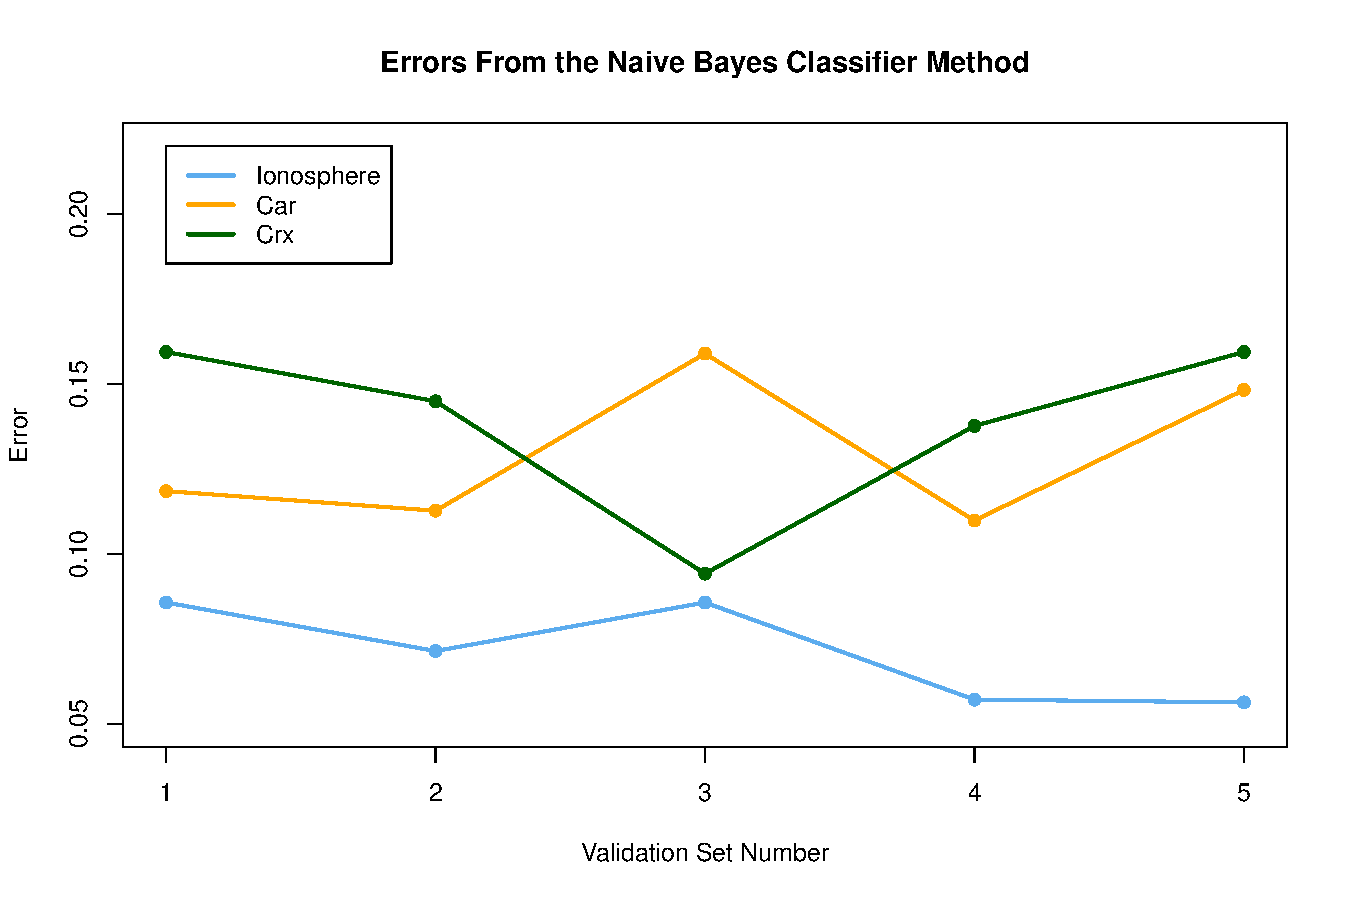
\includegraphics[width=0.9\linewidth]{Images/Prob3/Prob3-2-ErrPlot.pdf}
\end{center}
\bigskip

\bigskip





\qnum{3.3}\medskip

Now we compare the results from my implementation with results from using the \code{R} built-in implementation.

In the 3 graphs below, the \textcolor{blue}{\code{blue lines}} represent errors from using
\textcolor{blue}{\textbf{my implementation}} of the Naive Bayes Classifier, 
while the \textcolor{orange}{\code{orange dotted lines}} represent errors from using the
\textcolor{orange}{\textbf{R built-in implementation}}.

\begin{center}
    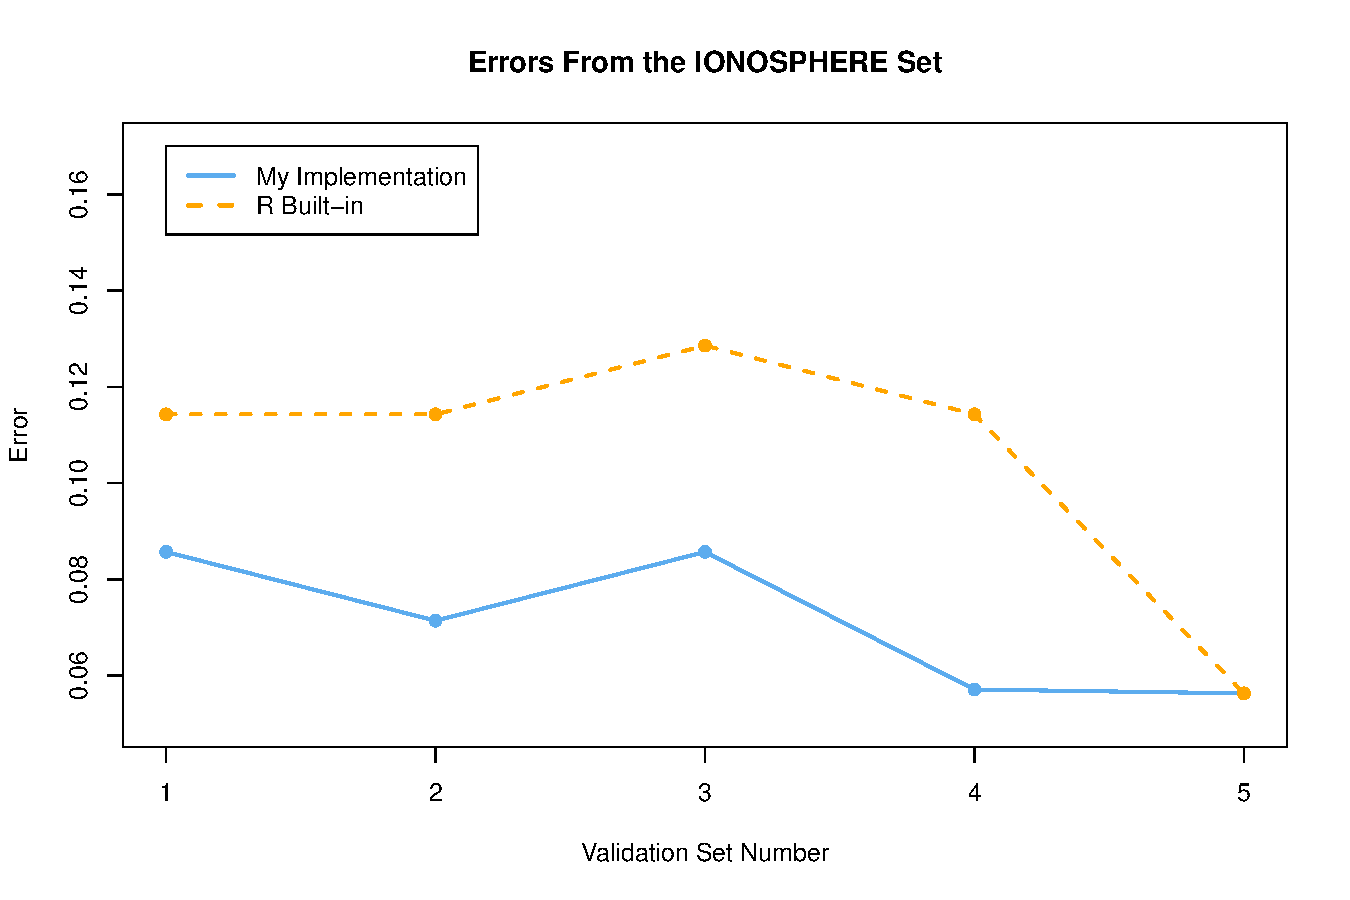
\includegraphics[width=0.9\linewidth]{Images/Prob3/Prob3-3-Iono.pdf}
    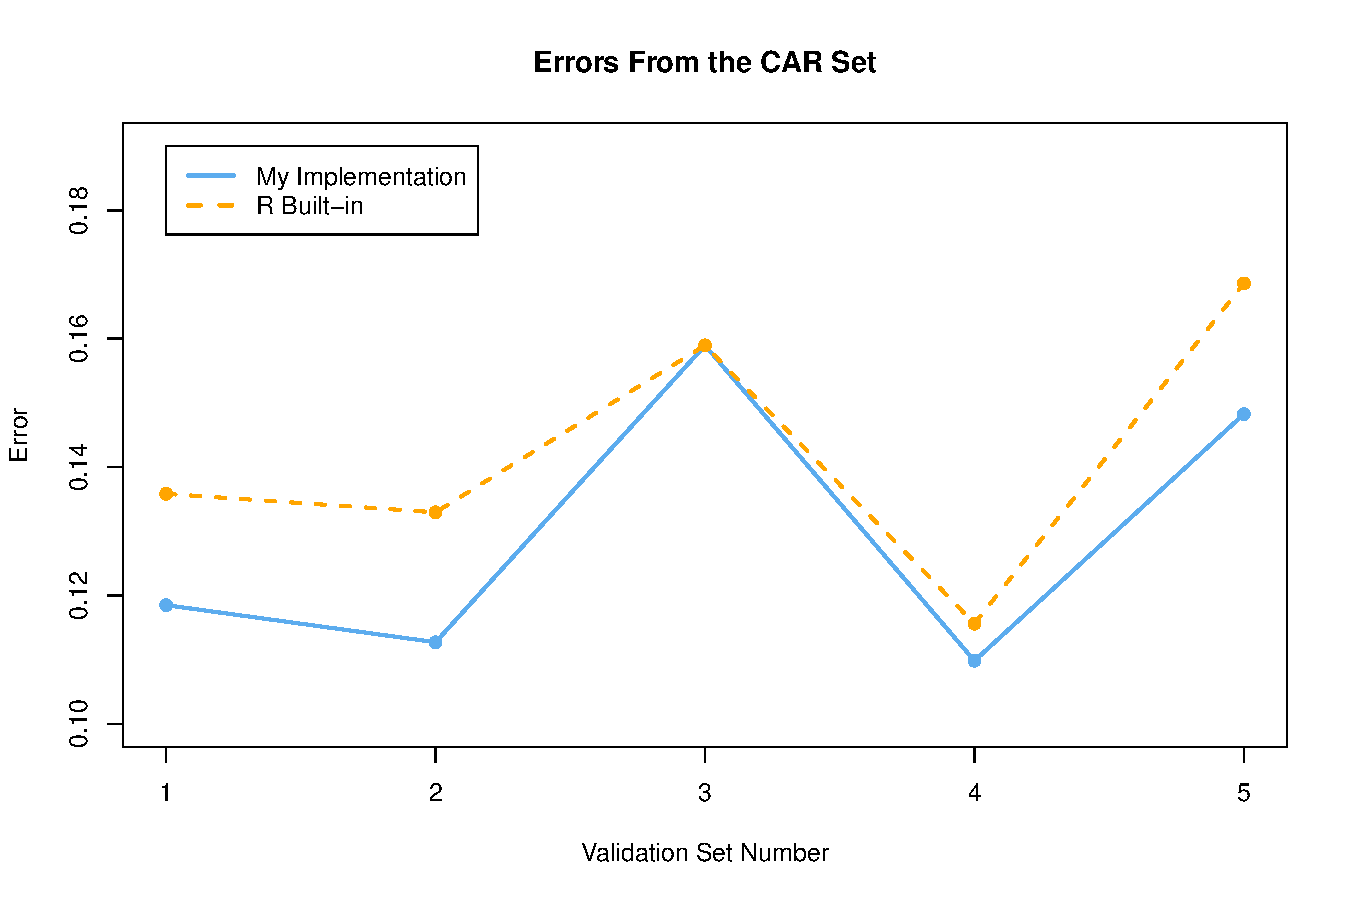
\includegraphics[width=0.9\linewidth]{Images/Prob3/Prob3-3-Car.pdf}
    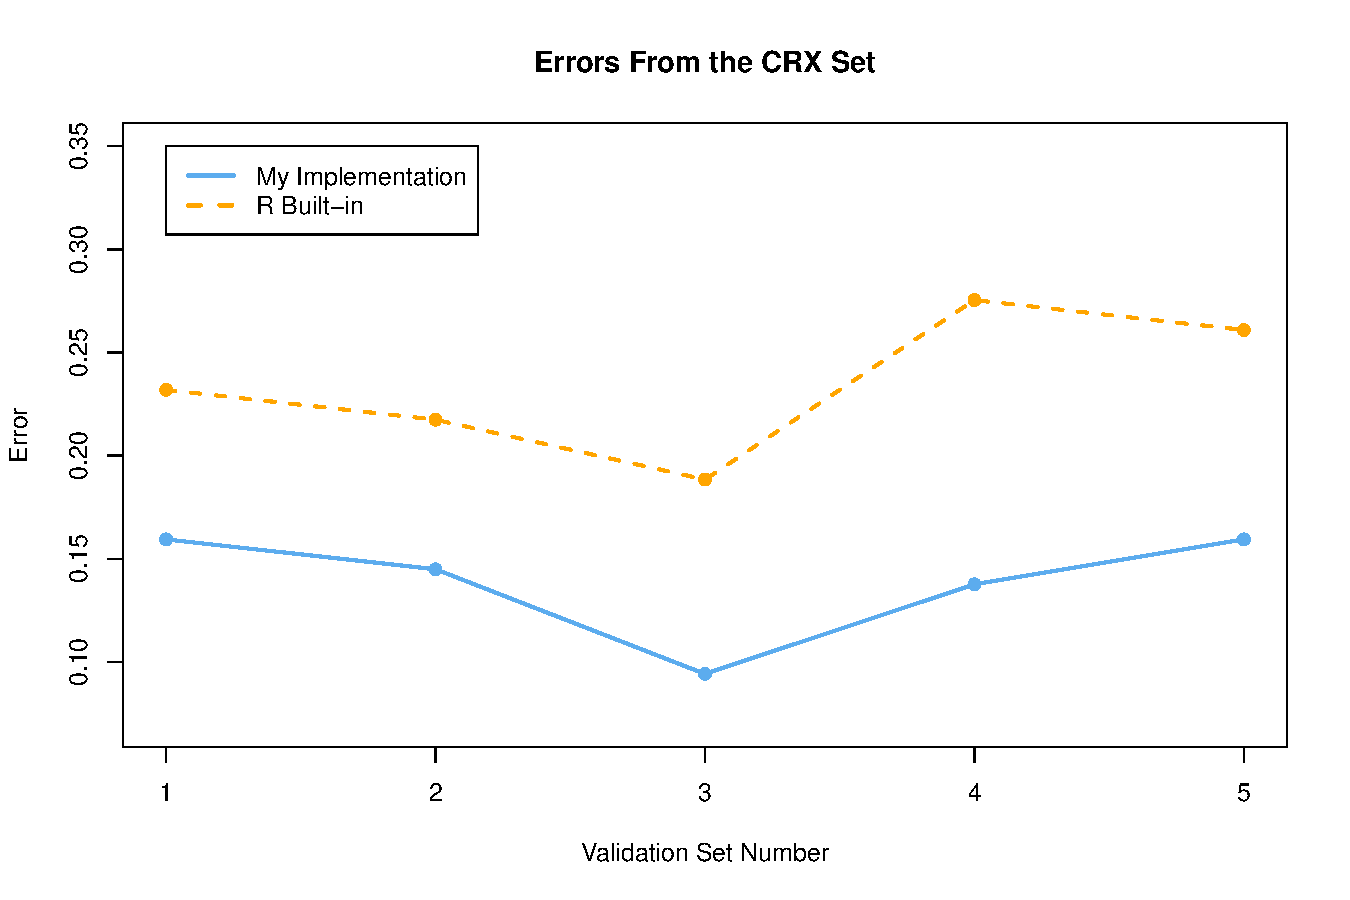
\includegraphics[width=0.9\linewidth]{Images/Prob3/Prob3-3-Crx.pdf}
\end{center}

Using the \code{R} built-in Naive Bayes Method, the average error rate is 0.1055533 for the Ionosphere set, 0.1423915 for the Car set, and 0.2347826 for the Crx set.
\bigskip


We can see from the error plots that, in general, our implementation of the Naive Bayes Classifier performs better than the \code{R} built-in implementation.

The difference is very pronounced in the \code{Ionosphere} and \code{Credit Approval Data} set, where continuous data exist. 
This is because, in our implementation, we hand picked the class-conditional distributions for the continuous features. For the continuous features, we make the distributional assumption of a normal distribution. But instead of directly using sample mean and variance as the distribution parameters, we experimented various parameter sets and chose the best parameters for each one of the \code{Ionosphere} and \code{Credit Approval Data} sets, using exploratory analysis. 
Note that for each data set, we have only one set of parameters for the distribution assumption, i.e. the parameters are the same across all validation sets.

The difference in the \code{Car} data set comes from the difference in the treatment of the categorical data. Converting categorical data using dummy variables improved our results. For the R experiments, we used the original data form, since Naive Bayes works with categorical data directly.
































%%%%%%%%%%%%%%%%%%%%%%%%%%%%%%%%%%%%%%%%%%%%%%%%%%%
%                        PROBLEM 4
%
%%%%%%%%%%%%%%%%%%%%%%%%%%%%%%%%%%%%%%%%%%%%%%%%%%%5
\newpage
\section*{Problem 4: Naive Bayes Classifier vs. $K$-Nearest Neighbors [30 points]} 

In this question, you are asked to compare Naive Bayes classifier with $k$-nn algorithm. First, determine the best KNN model for each data set. Then, Make a plot that reveals comparison of two algorithms using test error for each data set. (Total number of figures = 3)
\sep 

\noindent\textbf{Best Parameters for KNN}
\bigskip

For the Ionosphere data set, the best KNN method is using the 1-norm distance function with $k = 1$.

For the Car data set, the best KNN method is using the 1-norm distance function with $k = 1$.

For the Crx data set, the best KNN method is using the 1-norm distance function with $k = 13$.
\bigskip\bigskip



\noindent\textbf{Results Comparison}



\begin{center}
\newcommand{\cellISize}{3cm}
\newcommand{\cellIISize}{4cm}
\newcommand{\cellLastSize}{4.5cm}
\newcommand{\cellRowSize}{0.5cm}
\newcommand{\ci}[1]{\parbox{\cellISize}{\centering #1}}
\newcommand{\cii}[1]{& \parbox{\cellIISize}{\centering #1}}
\newcommand{\ciii}[1]{& \parbox{\cellLastSize}{\centering #1}}
\newcommand{\lineend}{&\\[\cellRowSize]\hline}
\textbf{Average Error Rate} 
\bigskip

\begin{tabular}{m{\cellISize} | m{\cellIISize} | m{4.0cm} m{0cm}}
    \toprule[1.5pt]
      \ci{\textbf{Data Set}}  
      \cii{\textbf{KNN}}
      \ciii{\textbf{Naive Bayes}}
      &\\[0.3cm]
    \midrule[0.8pt]
    %===== ===== ===== =====%
    \ci{Ionosphere} 
    \cii{0.08265594}
    \ciii{0.07126761}
    \lineend
    %===== ===== ===== =====%
    \ci{Car} 
    \cii{0.06769391}
    \ciii{0.1296512}
    \lineend
    %===== ===== ===== =====%
    \ci{Credit Approval} 
    \cii{0.1318841}
    \ciii{0.1391304}
    & \\[\cellRowSize]
    %===== ===== ===== =====%
    \bottomrule[1.5pt]
\end{tabular}
\end{center}
\bigskip



\begin{center}
    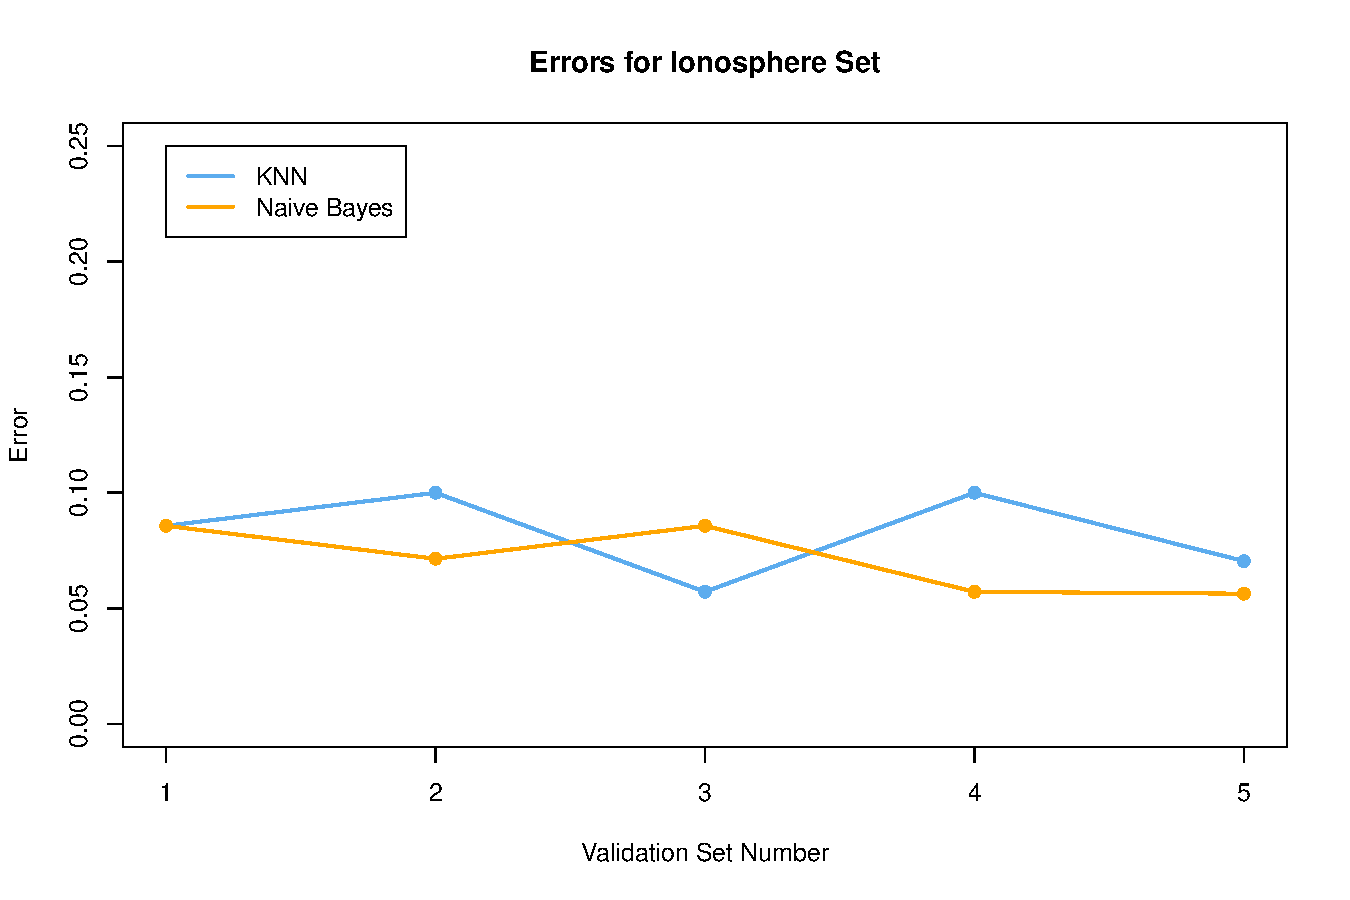
\includegraphics[width=0.75\linewidth]{Images/Prob4/Prob4-Iono.pdf}
    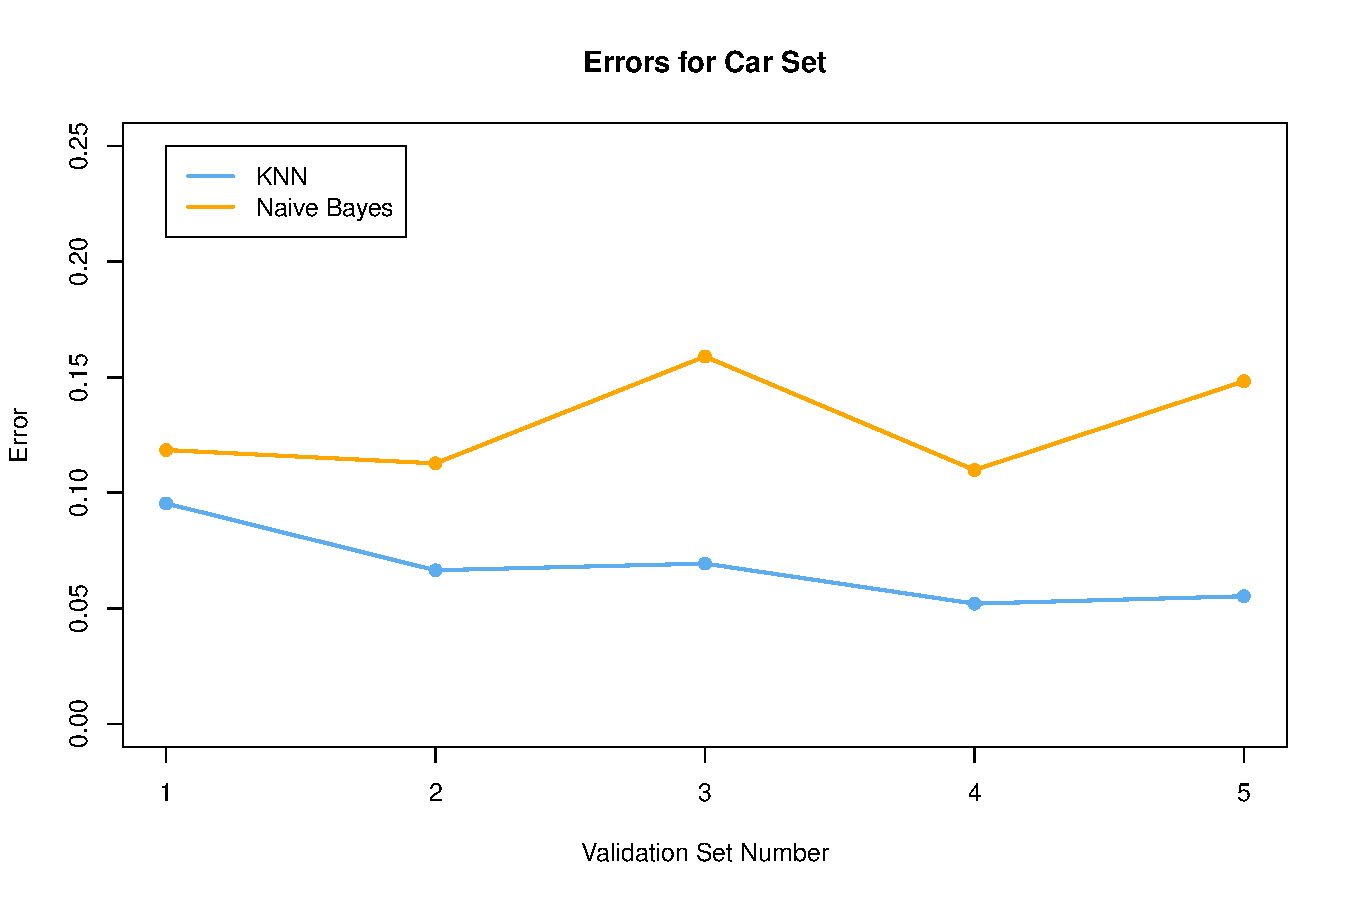
\includegraphics[width=0.75\linewidth]{Images/Prob4/Prob4-Car.pdf}
    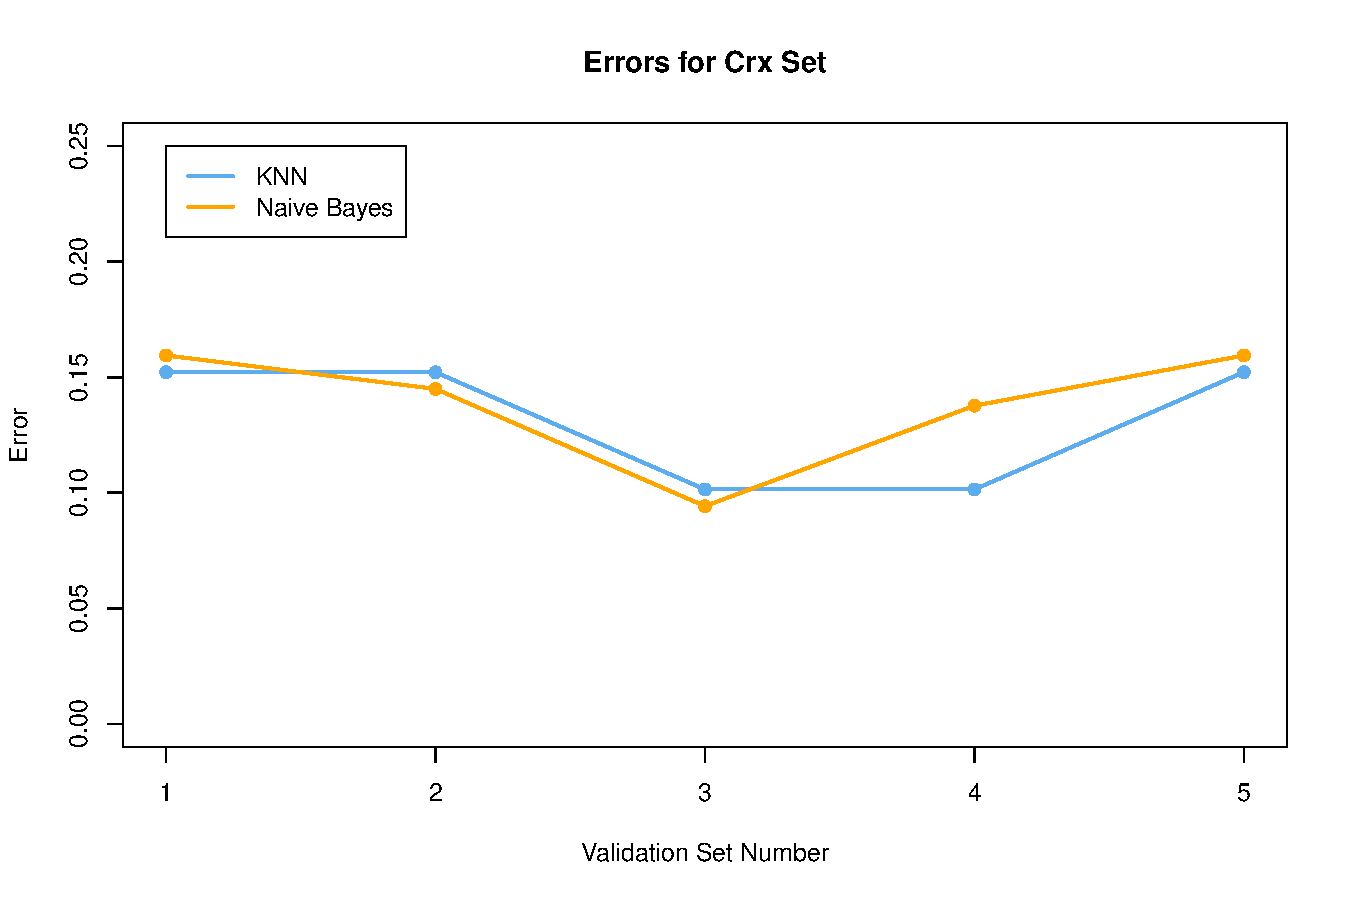
\includegraphics[width=0.75\linewidth]{Images/Prob4/Prob4-Crx.pdf}
\end{center}
\bigskip



\noindent\textbf{Conclusion}
\bigskip

From our implementations, the KNN method performs better than the Naive Bayes Classifier on the \code{Car} data set.
For the \code{Ionosphere} and \code{Credit Approval Data} sets, the two methods have similar performance on the test errors.
\bigskip











%%%%%%%%%%%%%%%%%%%%%%%%%%%%%%%%%%%%%%%%%%%%%%%%%%%
%                        PROBLEM 5
%
%%%%%%%%%%%%%%%%%%%%%%%%%%%%%%%%%%%%%%%%%%%%%%%%%%%5
\newpage
\section*{Problem 5 [15 points]} 

From textbook, Chapter 4 exercise  10.g and 13 (only for $k$-nn and logistic regression)
\sep 
\qnum{10g}

% trim={<left> <lower> <right> <upper>}
\begin{center}
    \textbf{Confusion Matrix}
    \bigskip
    
    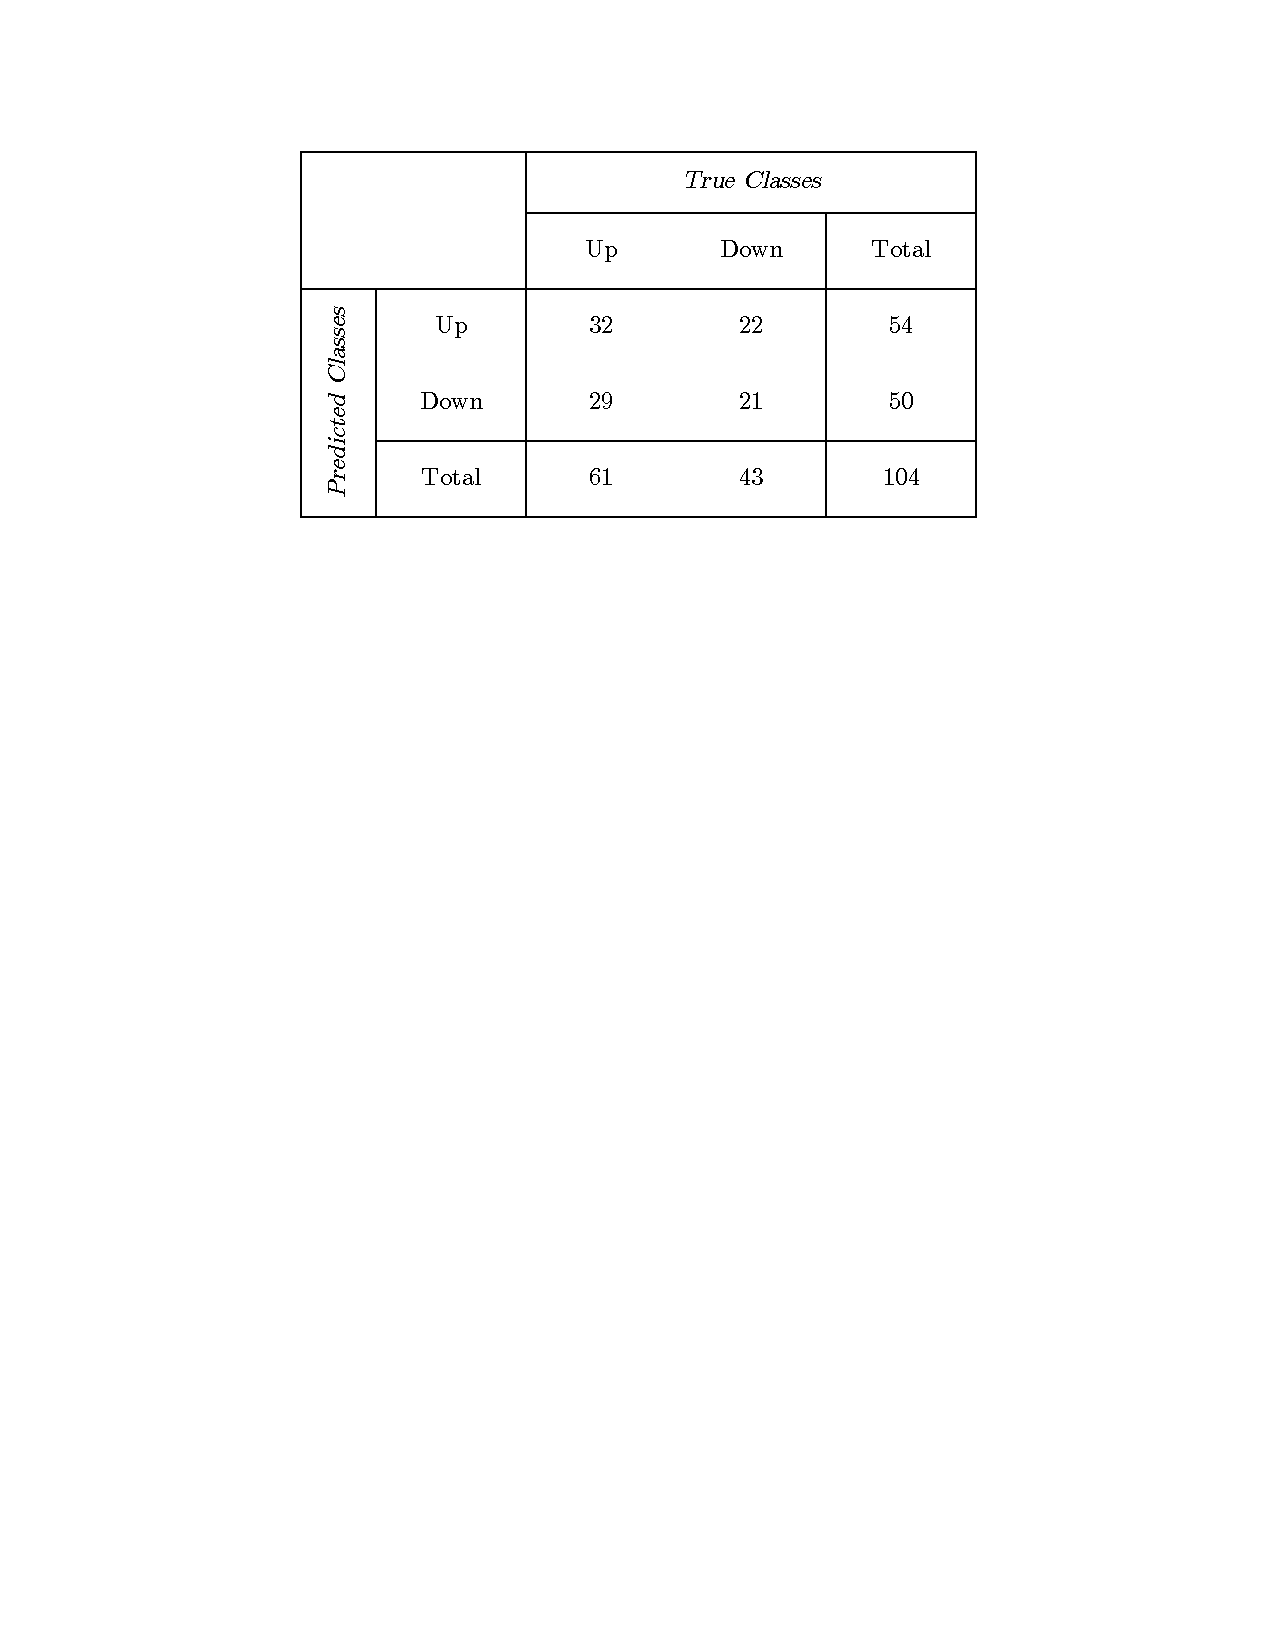
\includegraphics[trim={5cm 19cm 5cm 2.5cm},clip,width=0.55\linewidth]{Images/Prob5/Prob5-10-ConfMat.pdf}
\end{center}

The overall fraction of correct predictions for the held out data is 
\[
    \text{Fraction of correct predictions}
    = \frac{32 + 21}{104}
    = \frac{53}{104}
    \approx 0.5096154
\]
\bigskip\bigskip


\qnum{13}\medskip
\newcommand{\feat}[1]{\textcolor{myfirebrick}{\texttt{#1}}}

We experiment the following 6 subsets of predictors: subset 0, subset 1, $\cdots$, subset 5.
\bigskip


\noindent\textbf{Predictor Subset 0}
\[
    \begin{aligned}
    \text{predictor subset 0} =&\ 
    \{ 
    \feat{zn}, \feat{indus}, \feat{chas}, \feat{nox}, \feat{rm}, \feat{age}, \feat{dis},
              \feat{rad}, \feat{tax}, \feat{ptratio}, \feat{black}, \feat{lstat}, \feat{medv}
    \}\\
    =&\ \text{all features as predictors}
    \end{aligned}
\]

\begin{center}
    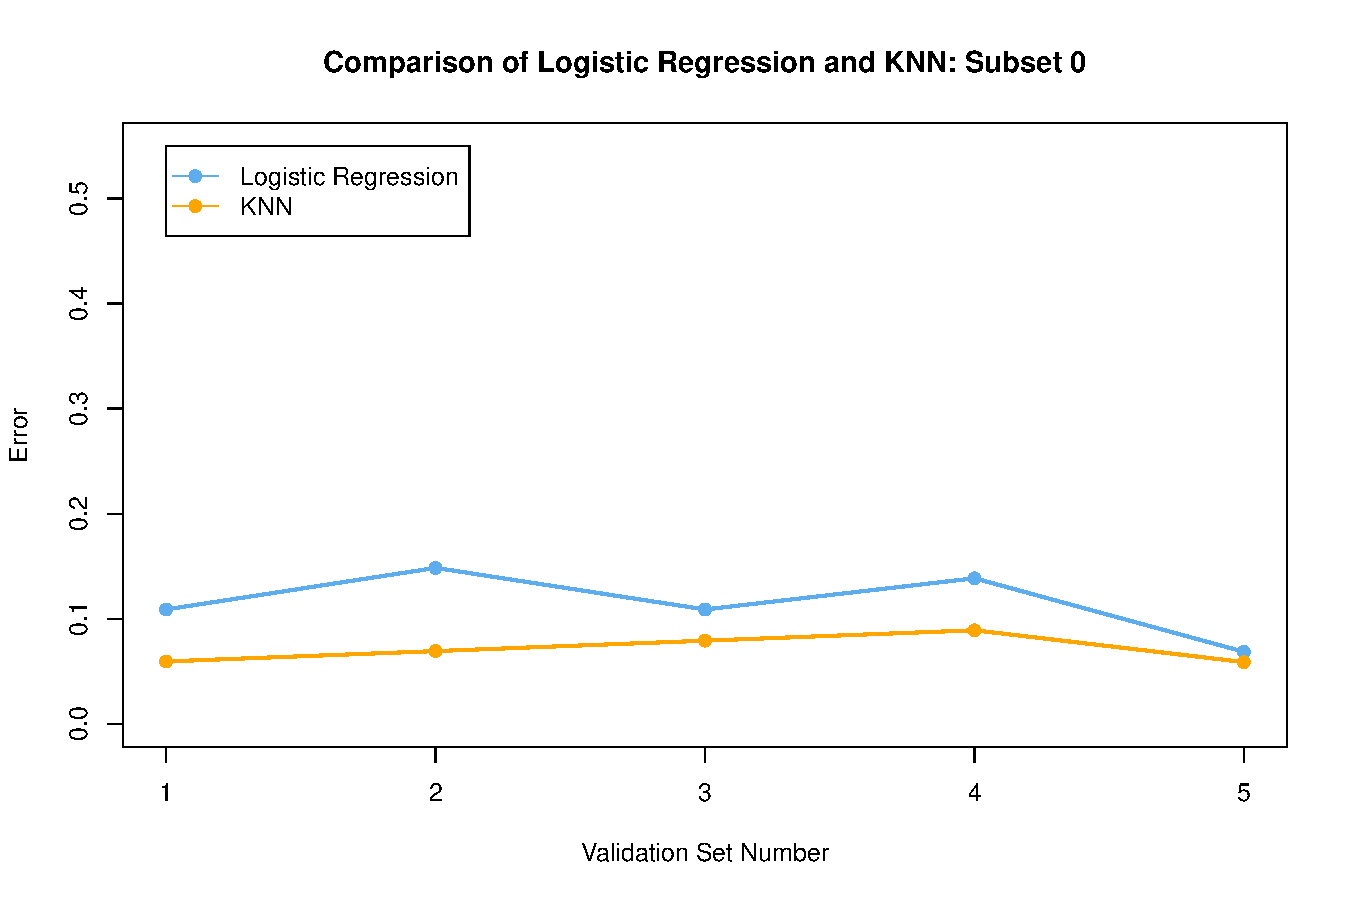
\includegraphics[width=0.8\linewidth]{Images/Prob5/Prob5-13-Plot-Subset0.pdf}
    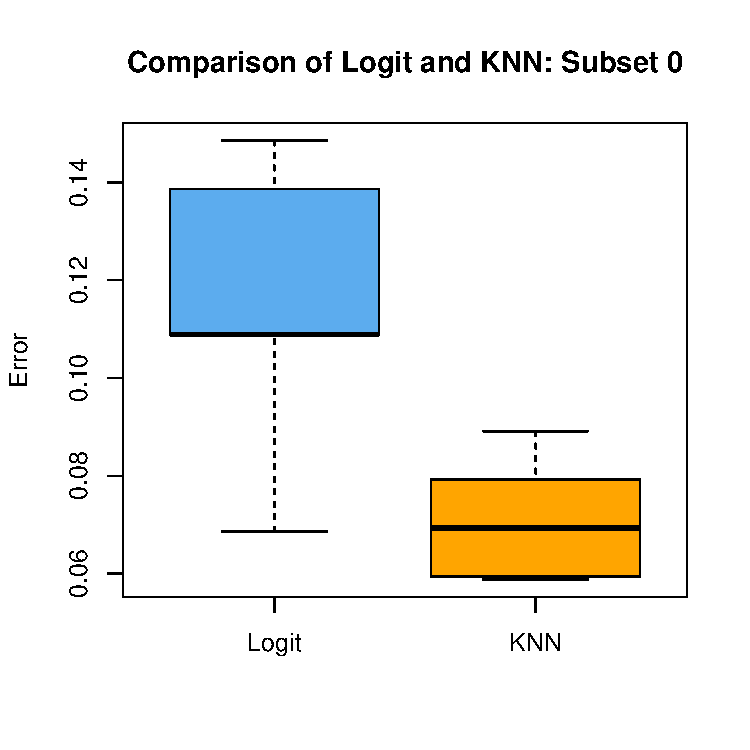
\includegraphics[width=0.45\linewidth]{Images/Prob5/Prob5-13-Boxplot-Subset0.pdf}
\end{center}

Using this subset of predictors, we can see that KNN performs better across the 5 validation sets. However, the difference in the performance of the logistic regression and KNN are not too different, compared to other subsets we experimented. In fact, as we can see below, this is the subset that the logistic regression performs the best.
\bigskip




\noindent\textbf{Predictor Subset 1}
\[
    \begin{aligned}
    \text{predictor subset 1} =&\ 
    \{ 
    \feat{zn}, \feat{indus}, \feat{chas}, \feat{nox}, \feat{rm}, \feat{age}, \feat{dis}
    \}
    \end{aligned}
\]

\begin{center}
    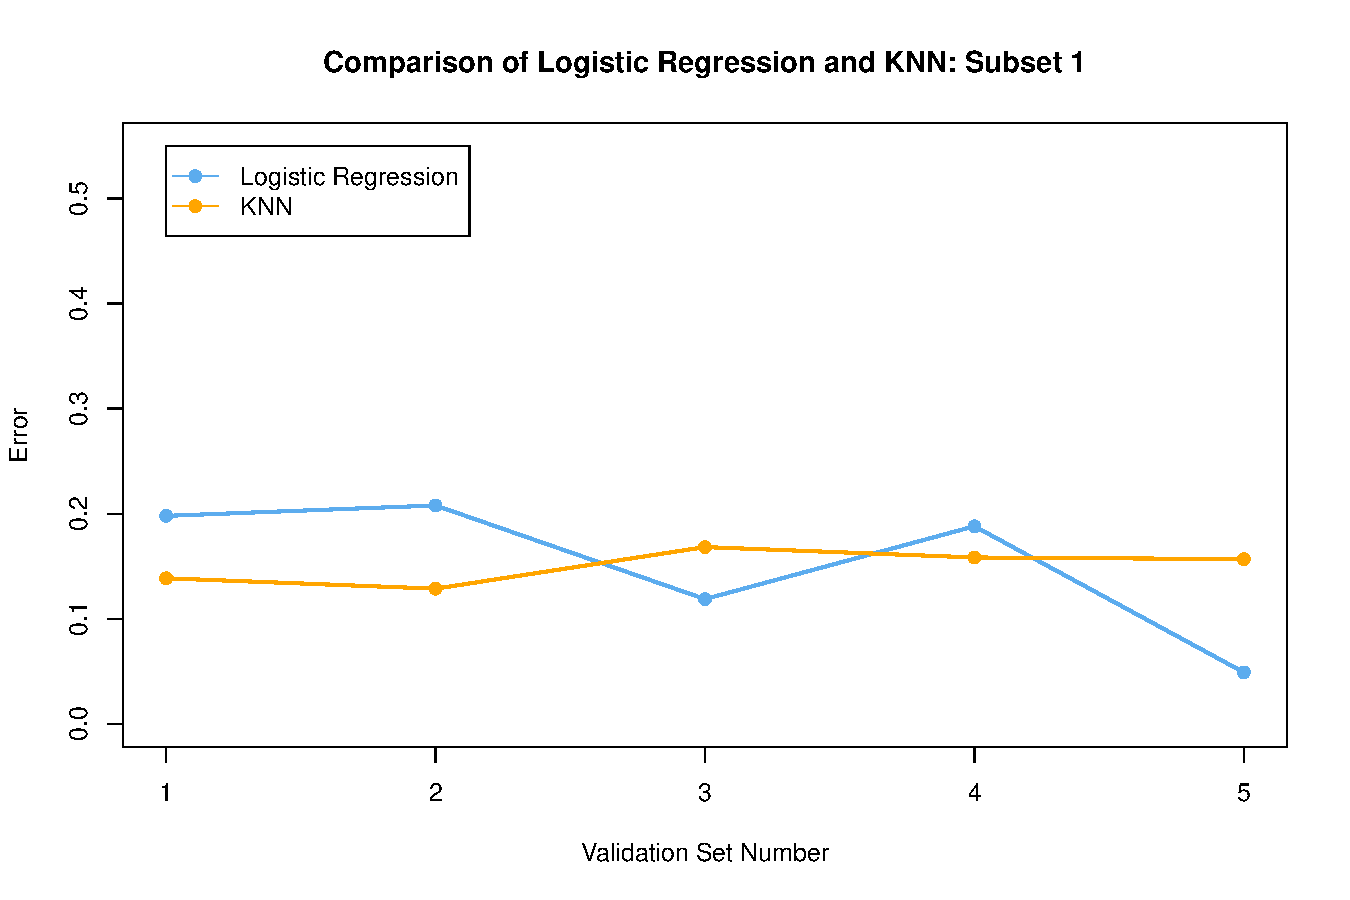
\includegraphics[width=0.8\linewidth]{Images/Prob5/Prob5-13-Plot-Subset1.pdf}
    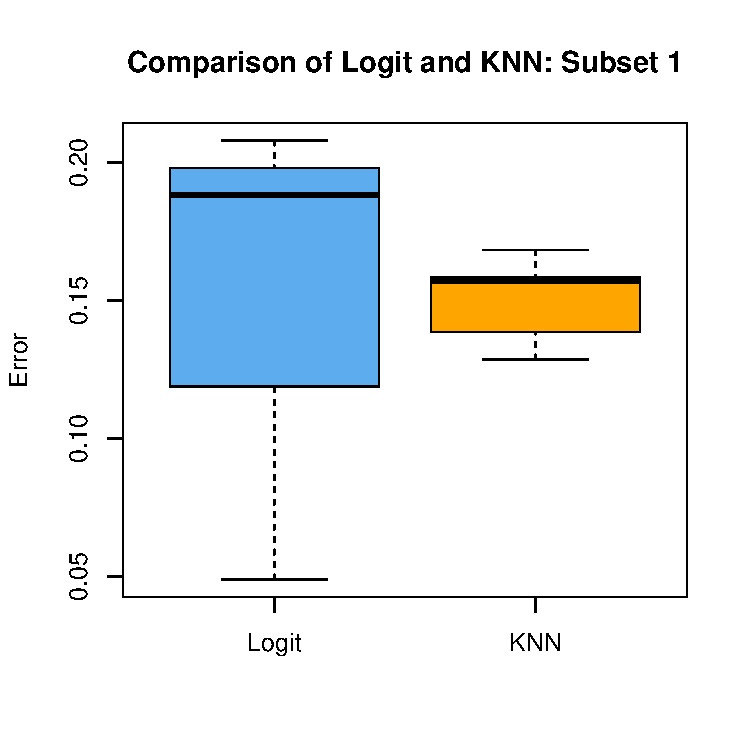
\includegraphics[width=0.45\linewidth]{Images/Prob5/Prob5-13-Boxplot-Subset1.pdf}
\end{center}

Using this subset of predictors, we can see that the performance of the logistic regression and KNN are similar, with KNN bringing better performance. 
However, neither of them gives very good error rates, with logit having average error rate of 0.1523782, and KNN having 0.1501844.
\bigskip




\noindent\textbf{Predictor Subset 2}
\[
    \begin{aligned}
    \text{predictor subset 2} =&\ 
    \{ 
        \feat{rad}, \feat{tax}, \feat{ptratio}, \feat{black}, \feat{lstat}, \feat{medv}
    \}
    \end{aligned}
\]


\begin{center}
    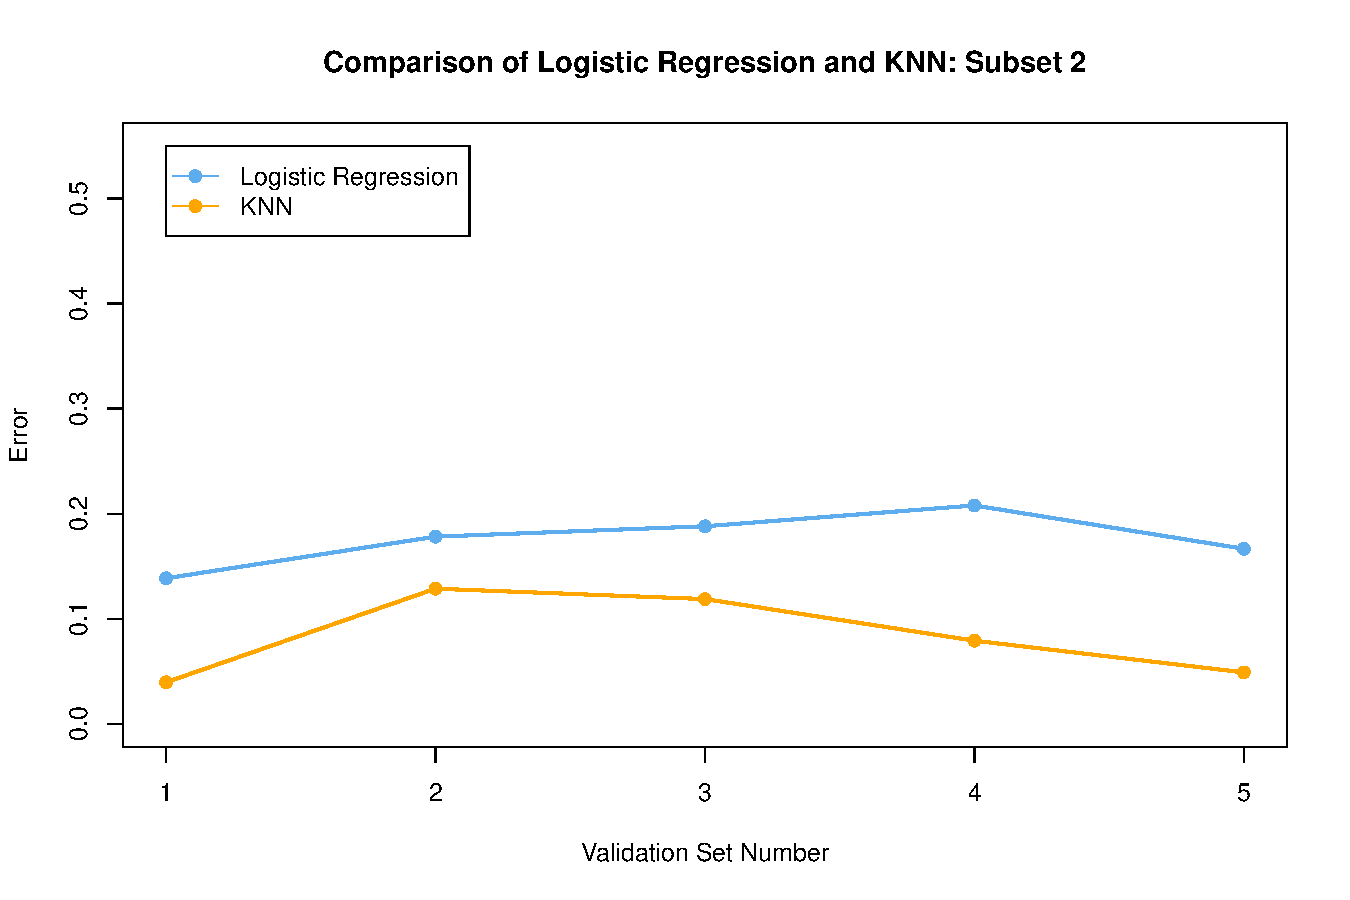
\includegraphics[width=0.8\linewidth]{Images/Prob5/Prob5-13-Plot-Subset2.pdf}
    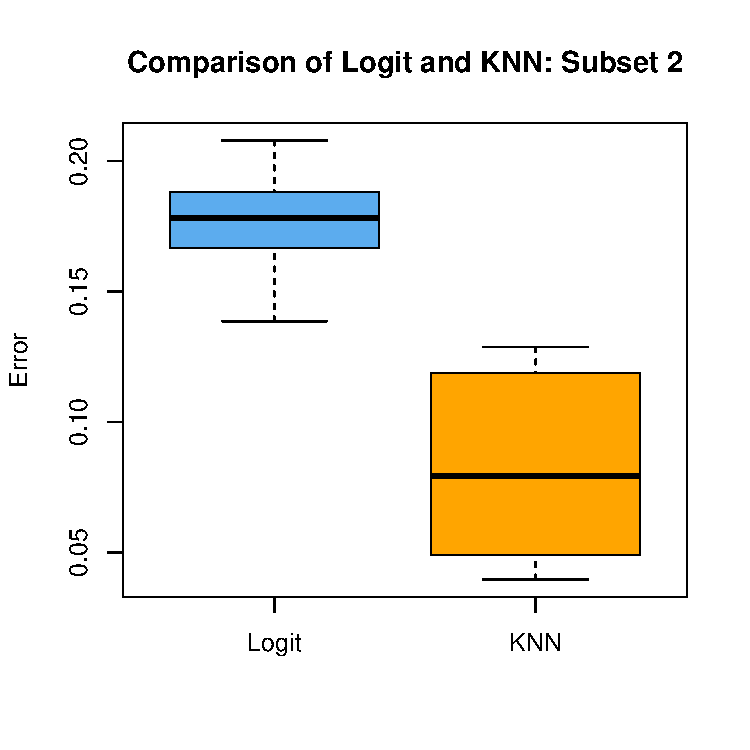
\includegraphics[width=0.45\linewidth]{Images/Prob5/Prob5-13-Boxplot-Subset2.pdf}
\end{center}

Using this subset of predictors, we can see that KNN performs better across the 5 validation sets, and it gives relatively low error rates, with average error rate being  0.08307126.
The logit results have higher error rates, with average error rate being 0.1759076.
\bigskip




\noindent\textbf{Predictor Subset 3}
\[
    \begin{aligned}
    \text{predictor subset 3} =&\ 
    \{ 
    \feat{zn}, \feat{chas}, \feat{rm}, \feat{dis},
              \feat{tax}, \feat{black}, \feat{medv}
    \}
    \end{aligned}
\]

\begin{center}
    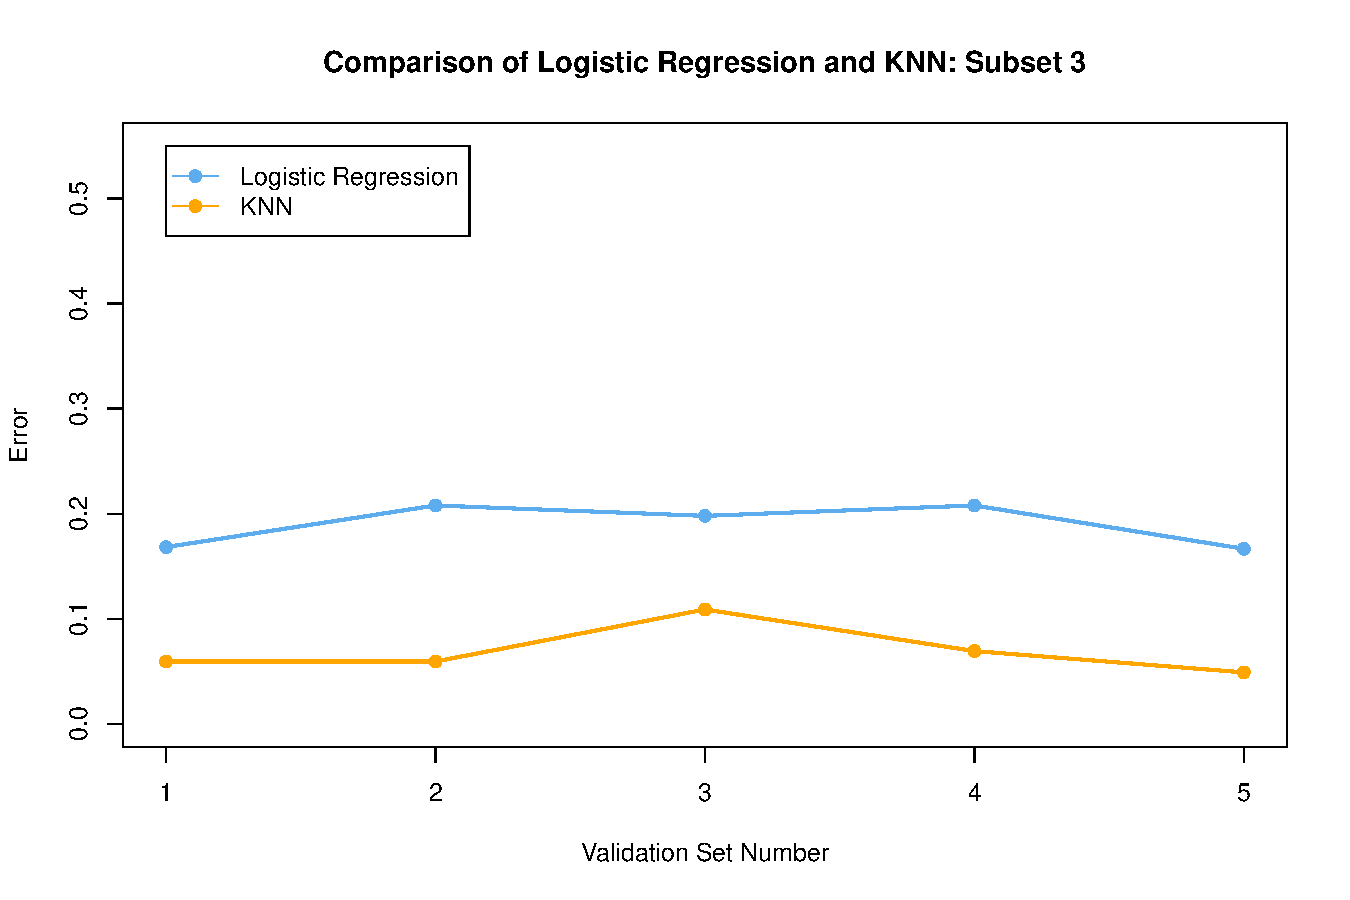
\includegraphics[width=0.8\linewidth]{Images/Prob5/Prob5-13-Plot-Subset3.pdf}
    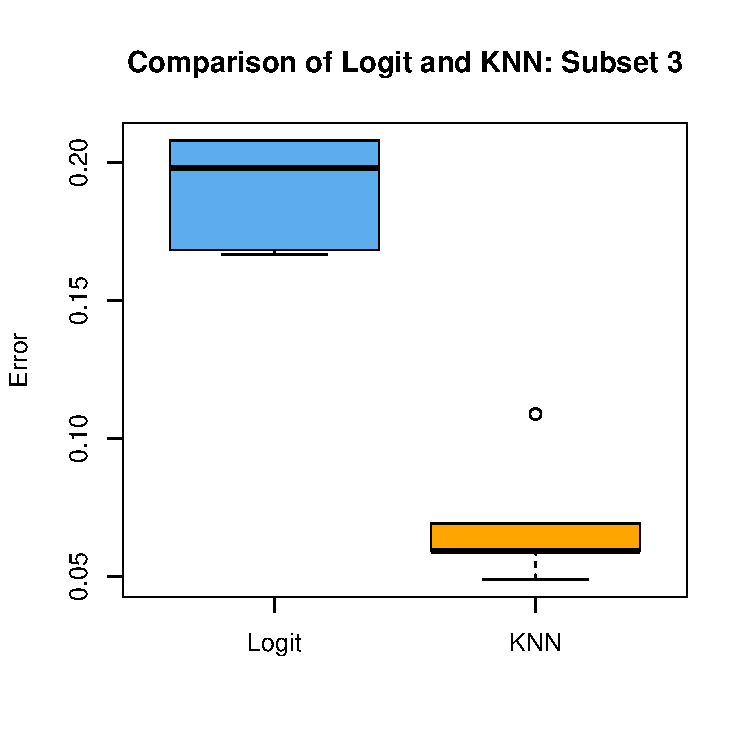
\includegraphics[width=0.45\linewidth]{Images/Prob5/Prob5-13-Boxplot-Subset3.pdf}
\end{center}

Using this subset of predictors, we can see that KNN performs better across the 5 validation sets. 
The KNN results are consistent on 5 validation sets and are relative low, with average error being 0.06920986.
The logit results are not very satisfactory, with average error being 0.189769.
\bigskip



\noindent\textbf{Predictor Subset 4}
\[
    \begin{aligned}
    \text{predictor subset 4} =&\ 
    \{ 
        \feat{tax}
    \}
    \end{aligned}
\]

\begin{center}
    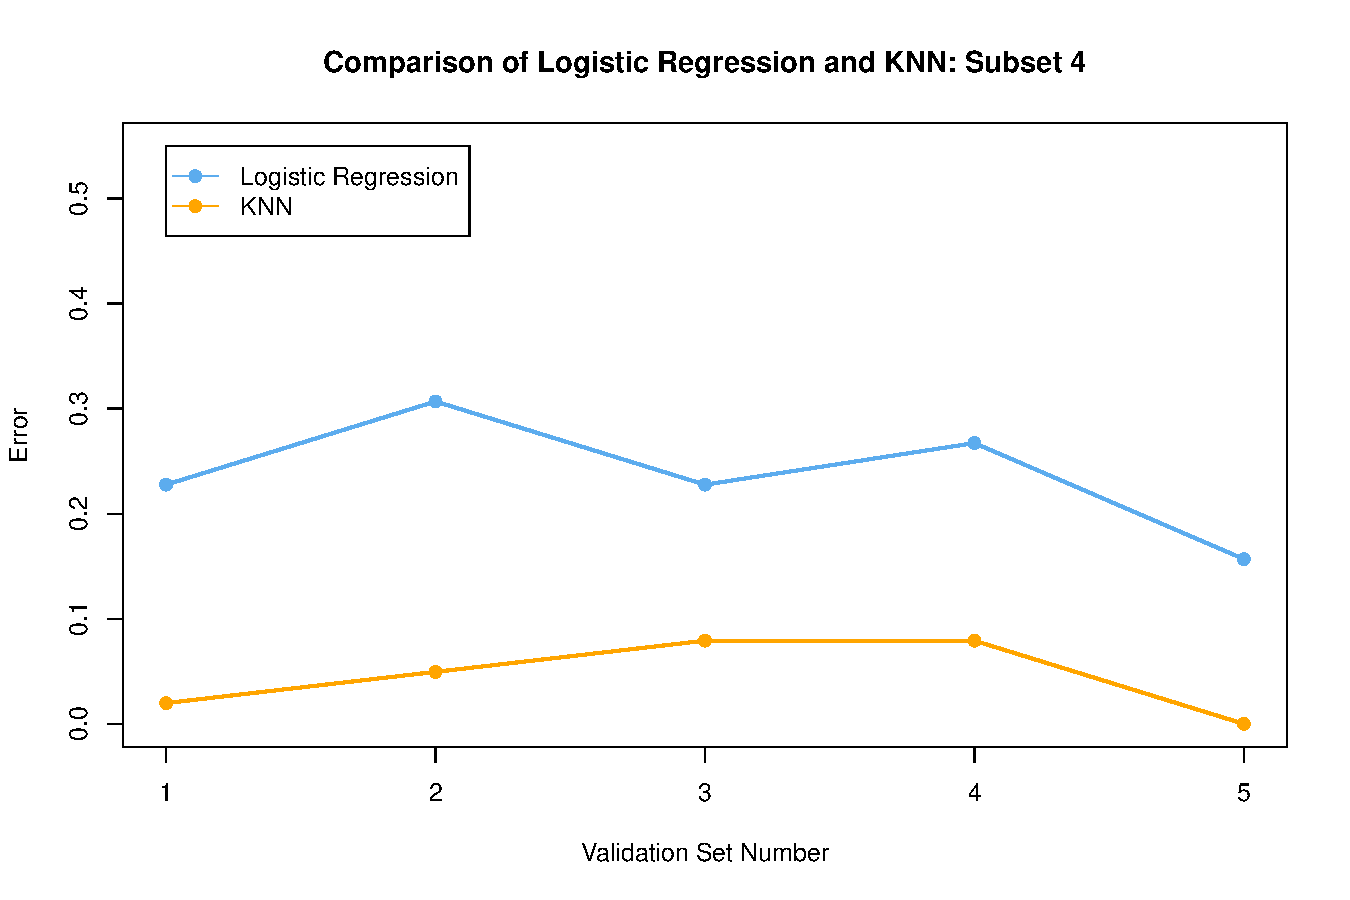
\includegraphics[width=0.8\linewidth]{Images/Prob5/Prob5-13-Plot-Subset4.pdf}
    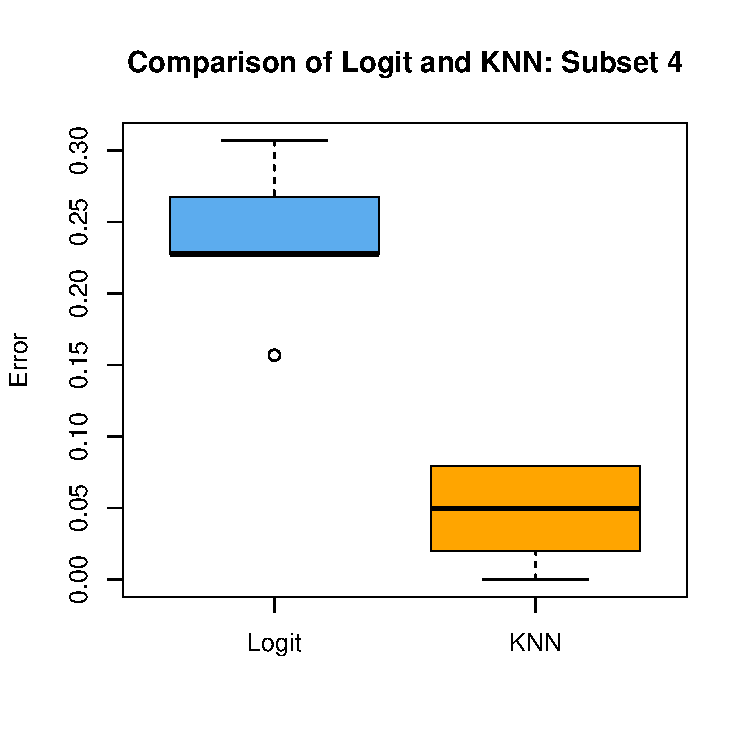
\includegraphics[width=0.45\linewidth]{Images/Prob5/Prob5-13-Boxplot-Subset4.pdf}
\end{center}

Using this subset of predictors, we can see that KNN performs better across the 5 validation sets. 
The KNN results are consistent on 5 validation sets and are relative low, with average error being 0.04554455.
The logit results are not very satisfactory, with average error being 0.2373131.
\bigskip




\noindent\textbf{Predictor Subset 5}
\[
    \begin{aligned}
    \text{predictor subset 5} =&\ 
    \{ 
        \feat{ptratio}
    \}
    \end{aligned}
\]

\begin{center}
    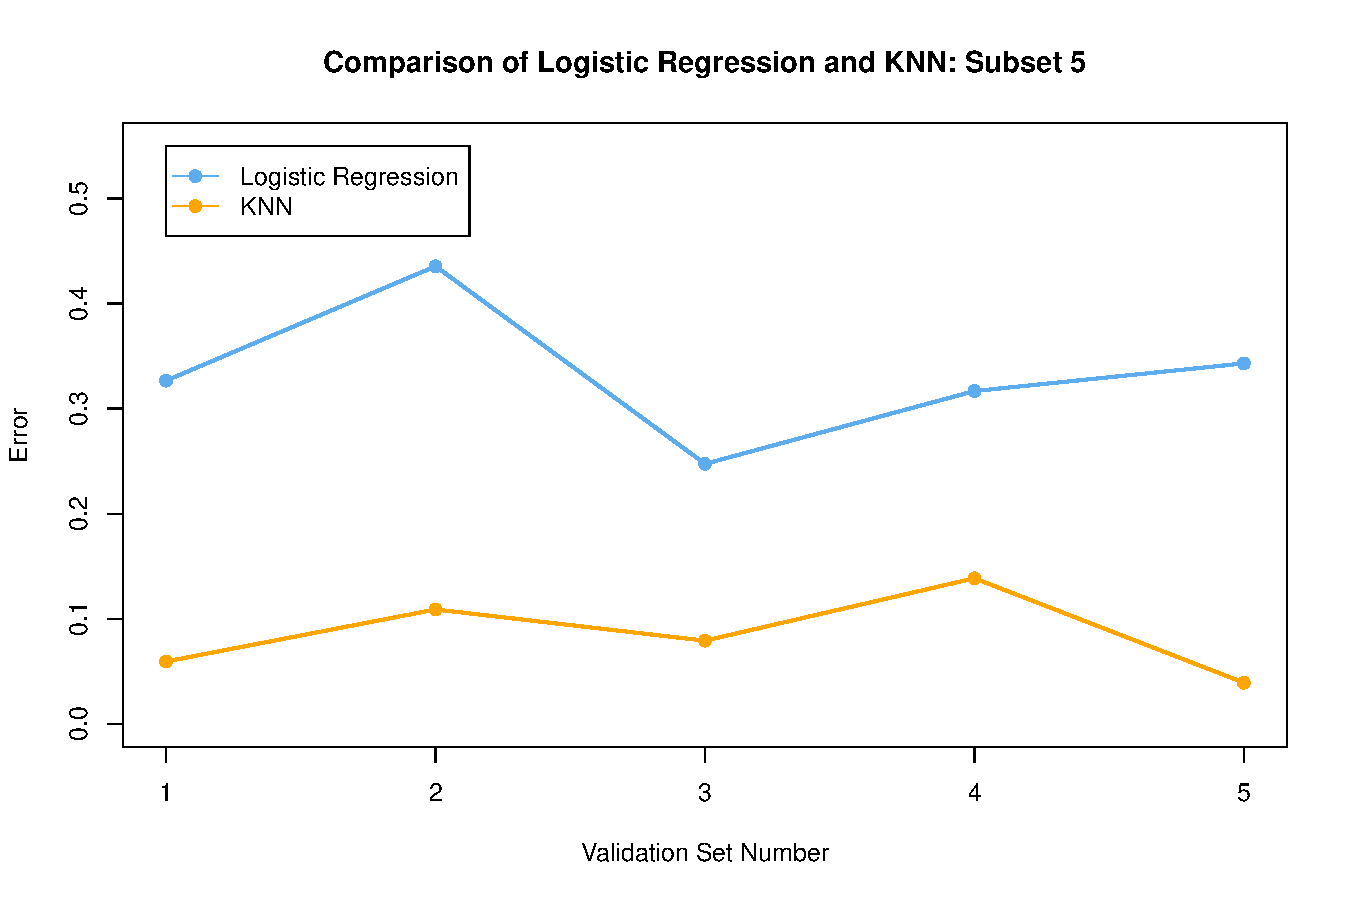
\includegraphics[width=0.8\linewidth]{Images/Prob5/Prob5-13-Plot-Subset5.pdf}
    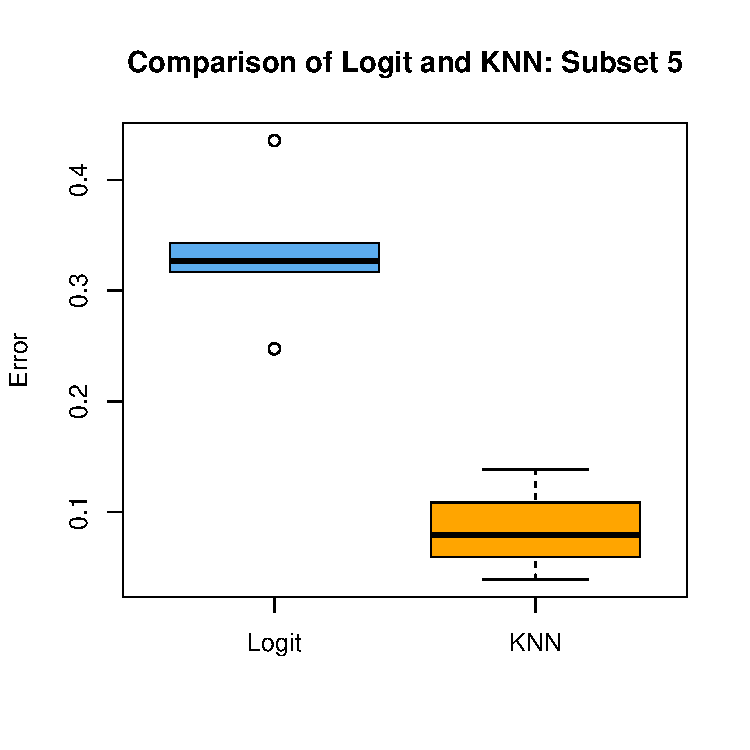
\includegraphics[width=0.45\linewidth]{Images/Prob5/Prob5-13-Boxplot-Subset5.pdf}
\end{center}

Using this subset of predictors, we can see that KNN performs better across the 5 validation sets. 
The KNN results are consistent on 5 validation sets and are relative low, with average error being 0.08507087.
The logit results are disappointing, with average error being 0.333974.
\bigskip\bigskip


\noindent\textbf{Conclusion}
\medskip

For all of the predictor subsets in our experiment, KNN performs better than logistic regression. 
The performance of logistic regression varies largely with the choice of the subset, while KNN brings good performance even with low number predictors.
This shows that this data set does not work as well with the logistic type of generalized linear model, as with the simpler model KNN. 


























%%%%%%%%%%%%%%%%%%%%%%%%%%%%%%%%%%%%%%%%%%%%%%%%%%%
%                       EXTRA
%
%%%%%%%%%%%%%%%%%%%%%%%%%%%%%%%%%%%%%%%%%%%%%%%%%%%5
\newpage
\section*{Extra credit (optional) [40 points]}

\begin{enumerate}
\item You are asked to evaluate the performance  of two classifier models, $M_1$ and $M_2$. The test set you have chosen contains 26 binary attributes, labeled as A through Z. The table below shows the posterior probabilities obtained by applying the models to the test set. (Only the posterior probabilities for the positive class are shown). As this is a two-class problem, P(-) = 1 - P(+) and P(-$|$A,\ldots,Z) = 1 - P(+$|$A,\ldots,Z). Assume that we are mostly interested in detecting instances from the positive class.

\begin{enumerate}
\item[(a)] Plot the ROC curve for both $M_1$ and $M_2$. Which model do you think is better. Explain your reasons? 

\item[(b)]  For model $M_1$, suppose you choose the cutoff threshold to be $t=0.5$. In other words, any test instances whose posterior probability is greater than $t$ will be classified as a positive example. Compute the precision, recall, and F-measure for the model at this threshold value.

\item[(c)] Repeat the analysis for part (c) using the same cutoff threshold on model $M_2$. Compare the F-measure results for both models. Which model is better? Are the results consistent with what you expect from the ROC curve? 


\item[(d)] Repeat part (c) for model $M_1$ using the threshold  
$t=0.1$. Which threshold do you prefer, $t=0.5$ or $t=0.1$? Are the results consistent with what you expect from ROC curve?

\end{enumerate}

\item Student/s who design/s the best either Naives Bayes classifier or KNN algorithm for the given data sets will receive  20 points.

\end{enumerate}
\sep

\qnum{a}
\begin{center}
    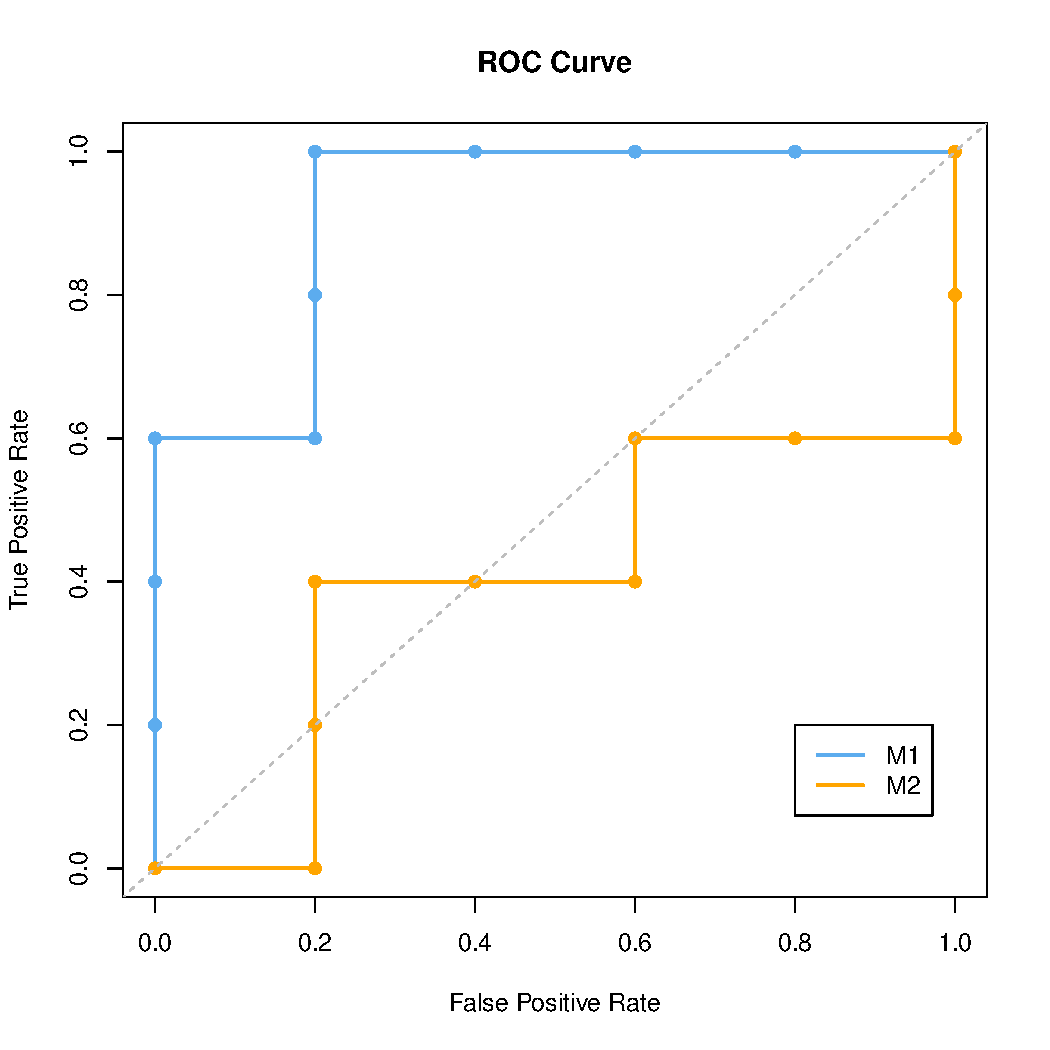
\includegraphics[width=0.6\linewidth]{Images/ProbEC-a-ROC.pdf}
\end{center}

The first model performs better.

We can see this by looking at the position of the curves. 
In this ROC curve, the top left area represents high true positive rate and low false positive rate, which the bottom right area represents low true positive rate and high false positive rate. Therefore, curves near the top left corner represents more desirable performance, while those near the bottom right corner represents poor performance. 

In our problem, the M1 curve hugs the top left corner. The M2 curve is entirely below the M1 curve and mostly locates below the diagonal line, towards the bottom right corner. Therefore, M1 performs better than M2.

Alternatively, we can look at the area under the curve or AUC. Obviously, M1 has larger AUC than M2. Therefore, M1 performs better than M2.
\bigskip












\newcommand{\TP}{\tx{TP}}
\newcommand{\FP}{\tx{FP}}
\newcommand{\TN}{\tx{TN}}
\newcommand{\FN}{\tx{FN}}

\qnum{b}
Using $t=0.5$, for model 1
\[
    \TP = 3,\quad 
    \FP = 1,\quad 
    \TN = 4,\quad 
    \FN = 2
\]
Therefore, 
\[
    \tx{precision} 
    = \frac{\TP}{\tx{P*}}
    =\frac{\TP}{\TP + \FP}
    = 0.75
\]

\[
    \tx{recall} 
    = \frac{\TP}{\tx{P}}
    =\frac{\TP}{\FN + \TP}
    = \frac{3}{2 + 3}
    = 0.6
\]

\[
    \tx{F-measure} 
    = 2\cdot \frac{\tx{precision}\cdot \tx{recall}}{\tx{precision} + \tx{recall}}
    = \frac{2}{3}
    \approx 0.6666667
\]
\bigskip



\qnum{c}
Using $t=0.5$, for model 2
\[
    \TP = 1,\quad 
    \FP = 1,\quad 
    \FN = 4
\]
Therefore, 
\[
    \tx{precision} 
    = \frac{\TP}{\tx{P*}}
    =\frac{\TP}{\TP + \FP}
    = \frac{1}{1 + 1}
    = 0.5
\]

\[
    \tx{recall} 
    = \frac{\TP}{\tx{P}}
    =\frac{\TP}{\FN + \TP}
    = \frac{1}{4 + 1}
    = 0.2
\]

\[
    \tx{F-measure} 
    = 2\cdot \frac{\tx{precision}\cdot \tx{recall}}{\tx{precision} + \tx{recall}}
    = \frac{2}{7}
    \approx 0.2857143
\]


Models with higher precision and recall, i.e. true positive rate, are considered to have the better performance.
The F-measure is the harmonic mean of precision and recall. Therefore, it is also positively correlated with model performance.

From the results above, we can see that all three scores, precision, recall and F-measure, are higher in model 1. Therefore, model 1 is better. This is consistent with the result from the ROC curve.  
\bigskip











\qnum{d}
Using $t=0.1$, for model 1
\[
    \TP = 5,\quad 
    \FP = 4,\quad 
    \TN = 1,\quad 
    \FN = 0
\]
Therefore, 
\[
    \tx{precision} 
    = \frac{\TP}{\tx{P*}}
    =\frac{\TP}{\TP + \FP}
    = \frac{5}{5 + 4}
    = \frac{5}{9}
    \approx 0.5555556
\]

\[
    \tx{recall} 
    = \frac{\TP}{\tx{P}}
    =\frac{\TP}{\FN + \TP}
    = \frac{5}{0 + 5}
    = 1
\]

\[
    \tx{F-measure} 
    = 2\cdot \frac{\tx{precision}\cdot \tx{recall}}{\tx{precision} + \tx{recall}}
    = \frac{5}{7}
    \approx 0.7142857
\]

From these scores, we can see that $t=0.1$ is better in recall or true positive rate, while $t=0.5$ is better in precision. Choosing either over the other would require some kind of trade-off. But if we use the F-measure to make the decision, we would choose $t=0.1$ over $t=0.5$, as it has a higher F-measure.

From the ROC, we can see that the point corresponding to $t=0.1$ for model 1 is 
$(0.8, 1)$,
the point corresponding to $t=0.5$ for model 1 is
$(0.2, 0.6)$. The conclusion we can draw is similar with the one we got from comparing precision, recall and F-measure values.


































\pagebreak
\section*{What to Turn-in (Submission Instructions)}

Put the below files in a zipped folder for your submission. The zipped folder should be named as \quotes{usename-section number}, i.e., hakurban-P556
\begin{enumerate}
\item The *tex and *pdf of the written answers to this document.
\item Code and Data
\begin{enumerate}
\item  Question 1: \textsf{crossValidation.R}, output of cross validation: training  and test data sets 
\item  Question 2.1: \textsf{knn.R}, Question 2.3: \textsf{knnValidation.R}
\item  Question 3.1: \textsf{naiveBayes.R}, Question 3.3: \textsf{naiveBayes-Validation.R}
\end{enumerate}
\item A README file that explains how to run your code and other files in the folder
\end{enumerate}























\bibliographystyle{plain}
\bibliography{ref} 

\end{document}


